\chapter{Валидация спектрального метода генерации синтетической турбулентности} \label{chapt4}

Одним из важных аспектов данной работы является программирование приведенных в главах \ref{chapt1} и \ref{chapt2}. Помимо того, что для достижения основной цели работы необходимо провести множество вычислений, необходимо также провести оптимизации алгоритмов, как для дальнейшего использования, так и для возможной конкуренции на рынке вычислительных пакетов и алгоритмов. Поэтому нужно уделить большее внимание данному аспекту. Помимо программирования основных методов, необходимо также реализовать сопутствующий функционал для валидации алгоритмов, а также удобного предоставления данных. Процесс можно разбить на несколько этапов. Первоначально, необходимо выбрать язык программирования для реализации алгоритмов. Следующим этапом проработать архитектуру приложения. В конечном итоге проводить вычислительные эксперименты.

Для выбора языка программирования, на котором будет вестись разработка, будут играть ключевую роль скорость, а также более простая интеграция с другими программами или сервисами. По первому признаку лучше всего подходят компилируемые языки программирования, дающие возможность получить наибольшую производительность. Наиболее популярным открытым пакетом для вычислительной гидродинамики является пакет "OpenFOAM". Для интеграции с "OpenFOAM" и различными библиотеками, например, линейной алгебры, наиболее лучшим вариантом становится выбор языка C или C++. Первый является подмножеством второго, выбор падает на C++ в силу предоставляемых языком программирования и его библиотекой стандартных примитивов, а также возможность интеграции с приведёнными выше пакетами. 

Тестирование алгоритмов проводилось на машине со следующими характеристиками:

\begin{enumerate}
	\item Процессор: Intel Core i5-13600KF (20 потоков, ~4.9 Ггц);
	\item RAM: Kingston Fury 4800 Мгц, 36-38-38-38;
	\item SSD накопитель: ADATA LEGEND 840 (чтение 5000 Мбайт/c, запись 3500 Мбайт/с);
\end{enumerate}

Компиляция программ для тестов и замеров производительности производилась с флагом максимальной оптимизации $O3$, без использования флага $ffast-math$ и подобных ему для ускорения работы с чилсами. Используемый тулчейн: $LLVM$ -- данная инфраструктура позволяет более безшовно производить кросс компиляцию проекта для разным операционных систем и архитектур процессоров.

Помимо реализации алгоритмов, необходимо реализовать также функционал связанный с расчётами статистических параметров, а также функционала для работы с сетками и вычислительными областями. Также необходимо реализовать функционал связанный с сохранением полученных данных для их дальнейшей обработки, таким образом можно сэкономить на памяти при выполнении дампов текущих параметров и полей. 

На данном, начальном этапе, пока будем реализовать функционал без интеграции с другими CFD пакетами, так как эта интеграция пока не требуется для валидации алгоритмов.

Также решено было реализовать варианты генерации синтетической турбулентности в виде библиотек для простоты дальнейшего использования, предоставляя программный интерфейс для генерации синтетической турбулентности для будущего пользователя. 

%
% Постановка задачи
%
Задачей является сгенерировать поле флуктуаций. Для турбулентного поля скоростей можно вычислить большое количество характеризующих его параметров, на данный момент нас в большей степени интересует спектр турбулентных флуктуаций. Спектр является главным входным параметром генерации, вследствие чего, вычисление его для результирующего поля, полученного в результате генерации, является основным критерием для оценки того или иного метода насколько он хорош для использования в качестве генератора турбулентных флуктуаций. С самим же спектром, в свою очередь, связано также достаточно много параметров. Например, как было описано ранее в главах \ref{chapt1} и \ref{chapt2}, спектр имеет связь как с тензором спектра скоростей, так и с тензором ковариаций. Последний является важной статистической величиной для оценки пространственной зависимости (корреляции) величин. Таким образом мы добавляем ещё один критерий валидации к поставленной задаче. 

Основное сравнение для спектрального метода будем проводить в сравнении с целевым спектром, так как в отличие от стохастического метода, мы отходим от энергетического спектра турбулентности. Как говорилось ранее, проводилась реализация метода Крайхнана, так как он является базисом для построения модификаций и других методов. Помимо этого сразу есть возможность выявить недостатки или преимущества данного метода по сравнению с модификациями вносимыми другими авторами. 

Так как метод сразу нацелен на генерацию трёхмерного поля скоростей будем рассматривать сразу все компоненты флуктуаций и результирующего спектра. 

Для генерации турбулентных флуктуаций на основе спектральных методов необходимо выделить основные физические парамеры для дальнейшего их переноса в программный код. Таким образом мы выделяем структуры данных, необходимые для реализации алгоритма. Основные соотношения и формулы позволяют выделить алгоритмы над упомянутыми ранее структурами данных как образами над физическими величинами. В отличие от метода стохастического Гауссового моделирования здесь имеется больше пространства как в плане количества рассматриваемых величин, так и в плане объема требуемых алгоритмов. По примеру Хуанга мы можем разбить целевой спектр в ряд, также будем рассматривать генерацию поля скоростей для случаев \ref{eq:spectral_equation3} дельта функции и Гауссового спектра. Первый случай позволяет использовать нам генератор на основе метода Крайхнана для генерации во всём интересующем диапазоне волновых чисел, второй в свою очередь для простого использования генератора в интервалах генерации и инерционном. Мы хотим использовать данные спектры чтобы не уходить от оригинальной постановки задачи и как можно более близко оставаться в рамках изначальных условий. Для одного экземпляра генератора нам необходимо сгенерировать последовательность волновых векторов в соответствии с процедурой генерации для каждого из спектров, для случая спектра дельта функции волновые вектора генерируются статистически изотропно на сфере заданного радиуса $k_0$, для случая гауссова спектра используется нормальное распределение со среднеквадратичным отклонением $\dfrac{k}{2}$. Дальше необходимо задаться некоторым значением среднеквадратичного отклонения для частоты $\omega_0$. Основное влияние эта частота оказывает на временную зависимость генерации синтетической турбулентности. В целом, способов задаться этой частотой достаточно много, авторы предлагают использовать $\omega_0 = k_0 v_0$, $v_0$ -- среднеквадратичное отклонение в любом направлении. Как можно легко убедиться комплекс $k_0 v_0$ имеет размерность частоты, а также может использоваться для перехода к безразмерному времени. Остается сгенерировать лишь амплитуды мод фурье, в оригинальной работе авторы не специфицируют алгоритм генерации, а точнее параметры генерации, данной последовательности случайных векторов. Но важно, что вектора амплитуд мод Фурье генерируются из трёхмерного нормального распределения. В данной работе мы использовали вариант со средним равным 0 и матрицей ковариации заданной единичной матрицей. Набор этих случайных величин генерируется всего один раз на этапе инициализации генератора и никак не привязан в топологии сетки. Важно отметить, что мы будем использовать разные экземпляр генератора для проведения одной реализации поля скоростей в начальный момент времени для оценки спектральных и статистических характеристик. Для оценки временных характеристик используется один экземпляр генератора с заранее заданным шагом генерации по времени. 
Всё это дает нам возможность использовать подход Хуанга для генерации синтетического поля скоростей с идей дискретизации спектра, а также в будущем заложить другую информацию, например о тензоре Рейнольдса в матрицу ковариаций генератора. 

Генерация случайных чисел проводлась с использованием генераторов случайных чисел, предоставляемых стандартной библиотекой шаблонов языка C++, для генерации многомерного Гауссова распределния использовалась библиотека "Armadillo". Генератор псевдослучайных чисел базируется на алгоритме Вихрь Мерсенна, показывающий более лучшие спектральные свойства по сравнению с генераторами Кнута и минимальный стандартным механизмом \cite{l2002object}, механизм Вихря Мерсенна имеет высокую производительность и хорошее качество генерируемых случайных чисел. Скорость работы генераторов является важной характеристикой, так как рассматриваемые алгоритмы полностью базируются на случайных числах. Функции распределения используемые в работе также использовались из стандартной библиотеки шаблонов С++ и библиотеки "Armadillo". 

Для удобства дальнейшей обработки данных будем генерировать поля флуктуаций на кубической сетке. Длину куба в параметрах будет обозначать $l$ и, как для рассматриваемого в данной главе метода, так и для стохастического метода, будем брать $l = 10$, пока без введения конкретной размерности. Также сетка характеризуется числом разбиений по каждой из осей, будем использовать одинаковое число разбиений для каждой из осей $n_x = n_y = n_z = n$. Число разбиений будем использовать максимально доступное для вычислений на машине с объемом оперативной памяти в 32 Гб. Данный метод имеет хорошую устойчивость к топологии сетки, то-есть не зависит от расположения соседних узлов, её формы, поэтому можно с большой достоверностью считать, что использование данной сетки обосновано для проведения валидации получаемых данных. Для простоты также центр куба будет совпадать с началом координат, так будет проще оценить симметричность функций относительно точки расчёта статистических параметров, которую также примем за начало координат, в этом случае $R_{ij}(\vec x, \vec r) = \left< u_i(\vec x) u_j(\vec x + \vec r) \right> \rightarrow \left[ \vec x = {0, 0, 0} \right] \rightarrow R_{ij}(\vec r) = \left< u_i(\vec 0) u_j(\vec 0 + \vec r) \right>$. Важность оценки симметричности функции играет важную роль при переходе от тензора ковариаций к тензору спектра скоростей, так как это необходимое условие для проведения преобразования Фурье

Далее будут представлены сгенерированные поля в момент времени $t = 0$ для $k_0 = \frac{\pi}{3}$, $n = 31$, $v_0 = 1$, $\omega_0 = v_0 k_0 = 2 \pi$, для спектра в виде дельта-функции. Для проведения статистического анализа, а также дальнейшего вычисления тензора спектра скоростей и энергетического спектра генерируется $N_{samples} = 10000$, в 10 раз больше взятого числа мод Фурье, которое составляет $N = 1000$. 

\begin{figure}[!h]
    \center{
        \hfill
        \subcaptionbox[List-of-Figures entry]{Полное сгенерированное поле\label{img:spectral_slice_veloctiy_field_full_cube}} 
        {\includegraphics[width=0.4\linewidth]{images/spectral/spectral_n32_l10_f1000_k0pi3/full_velocity_field_cube_spectral.png}}%
        \hfill       
        \subcaptionbox{плоскость $xy$, $z = 0$\label{img:spectral_slice_veloctiy_field_x_znormal_angle_trace}} 
        {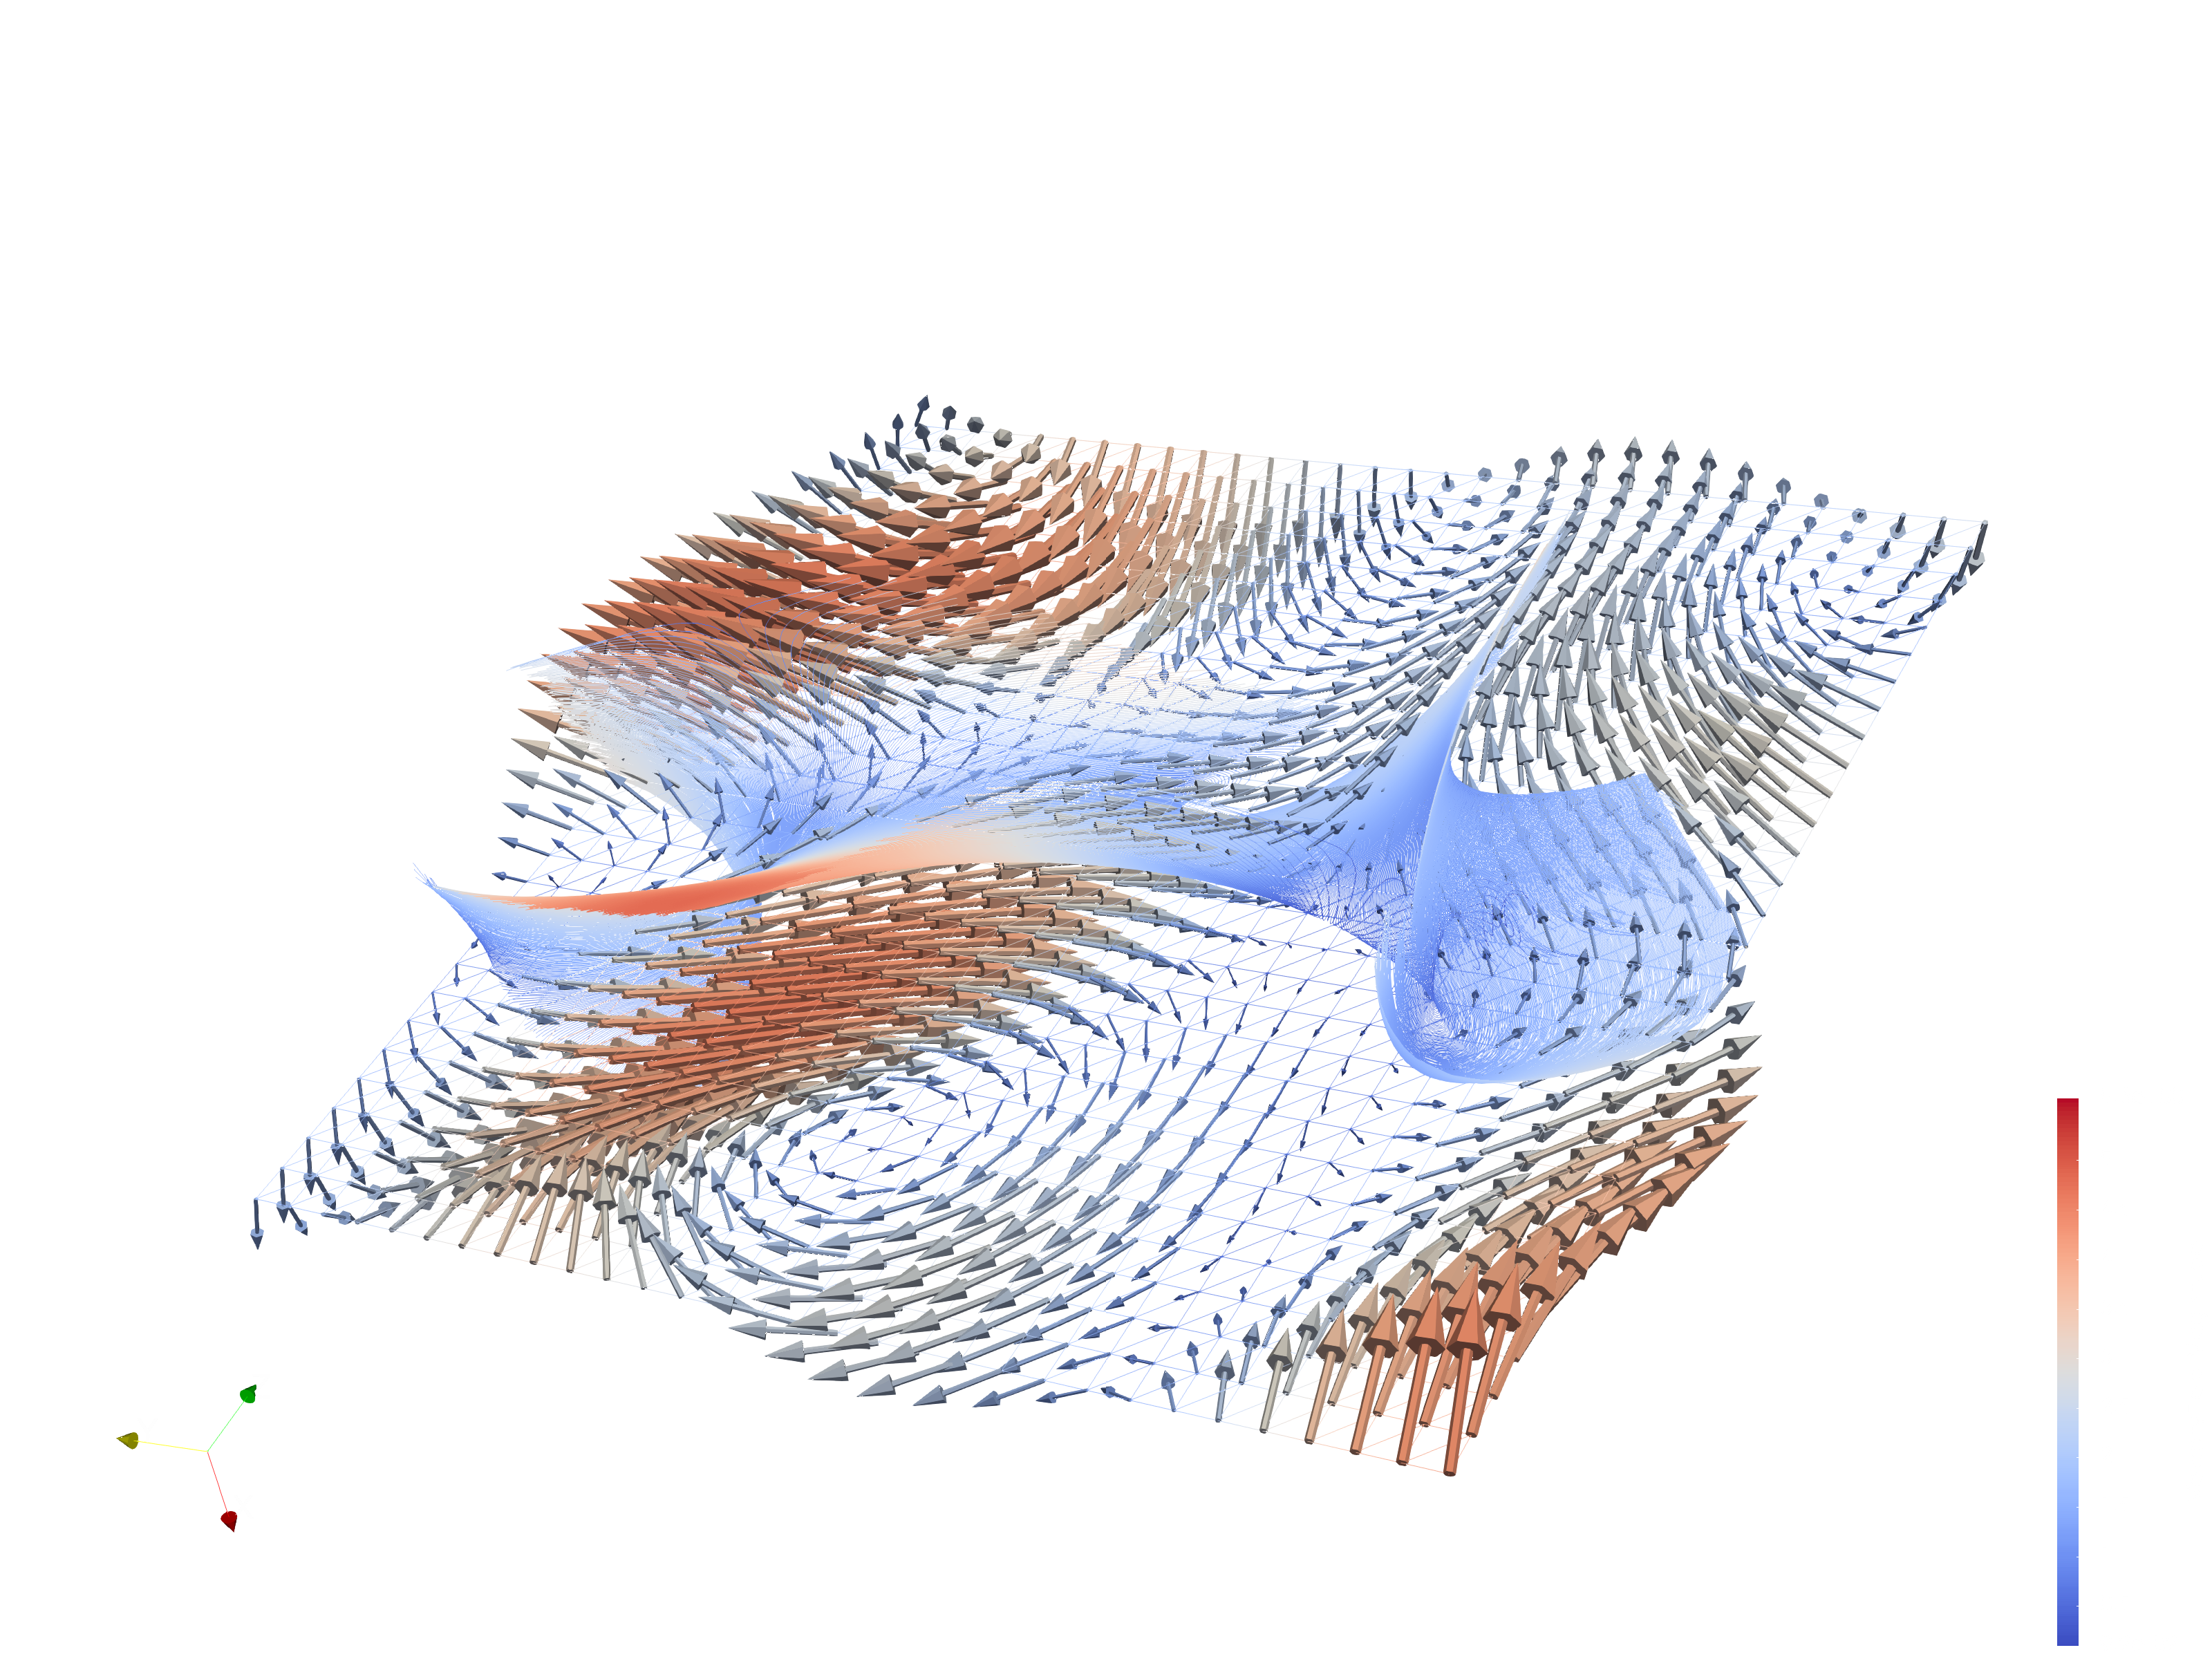
\includegraphics[width=0.4\linewidth]{images/spectral/spectral_n32_l10_f1000_k0pi3/spectral_x_normal_velocity_field_angle_trace.png}} \\
        \hfill
        \subcaptionbox[List-of-Figures entry]{плоскость $xy$, $z = 0$\label{img:spectral_slice_veloctiy_field_x_znormal_angle}} 
        {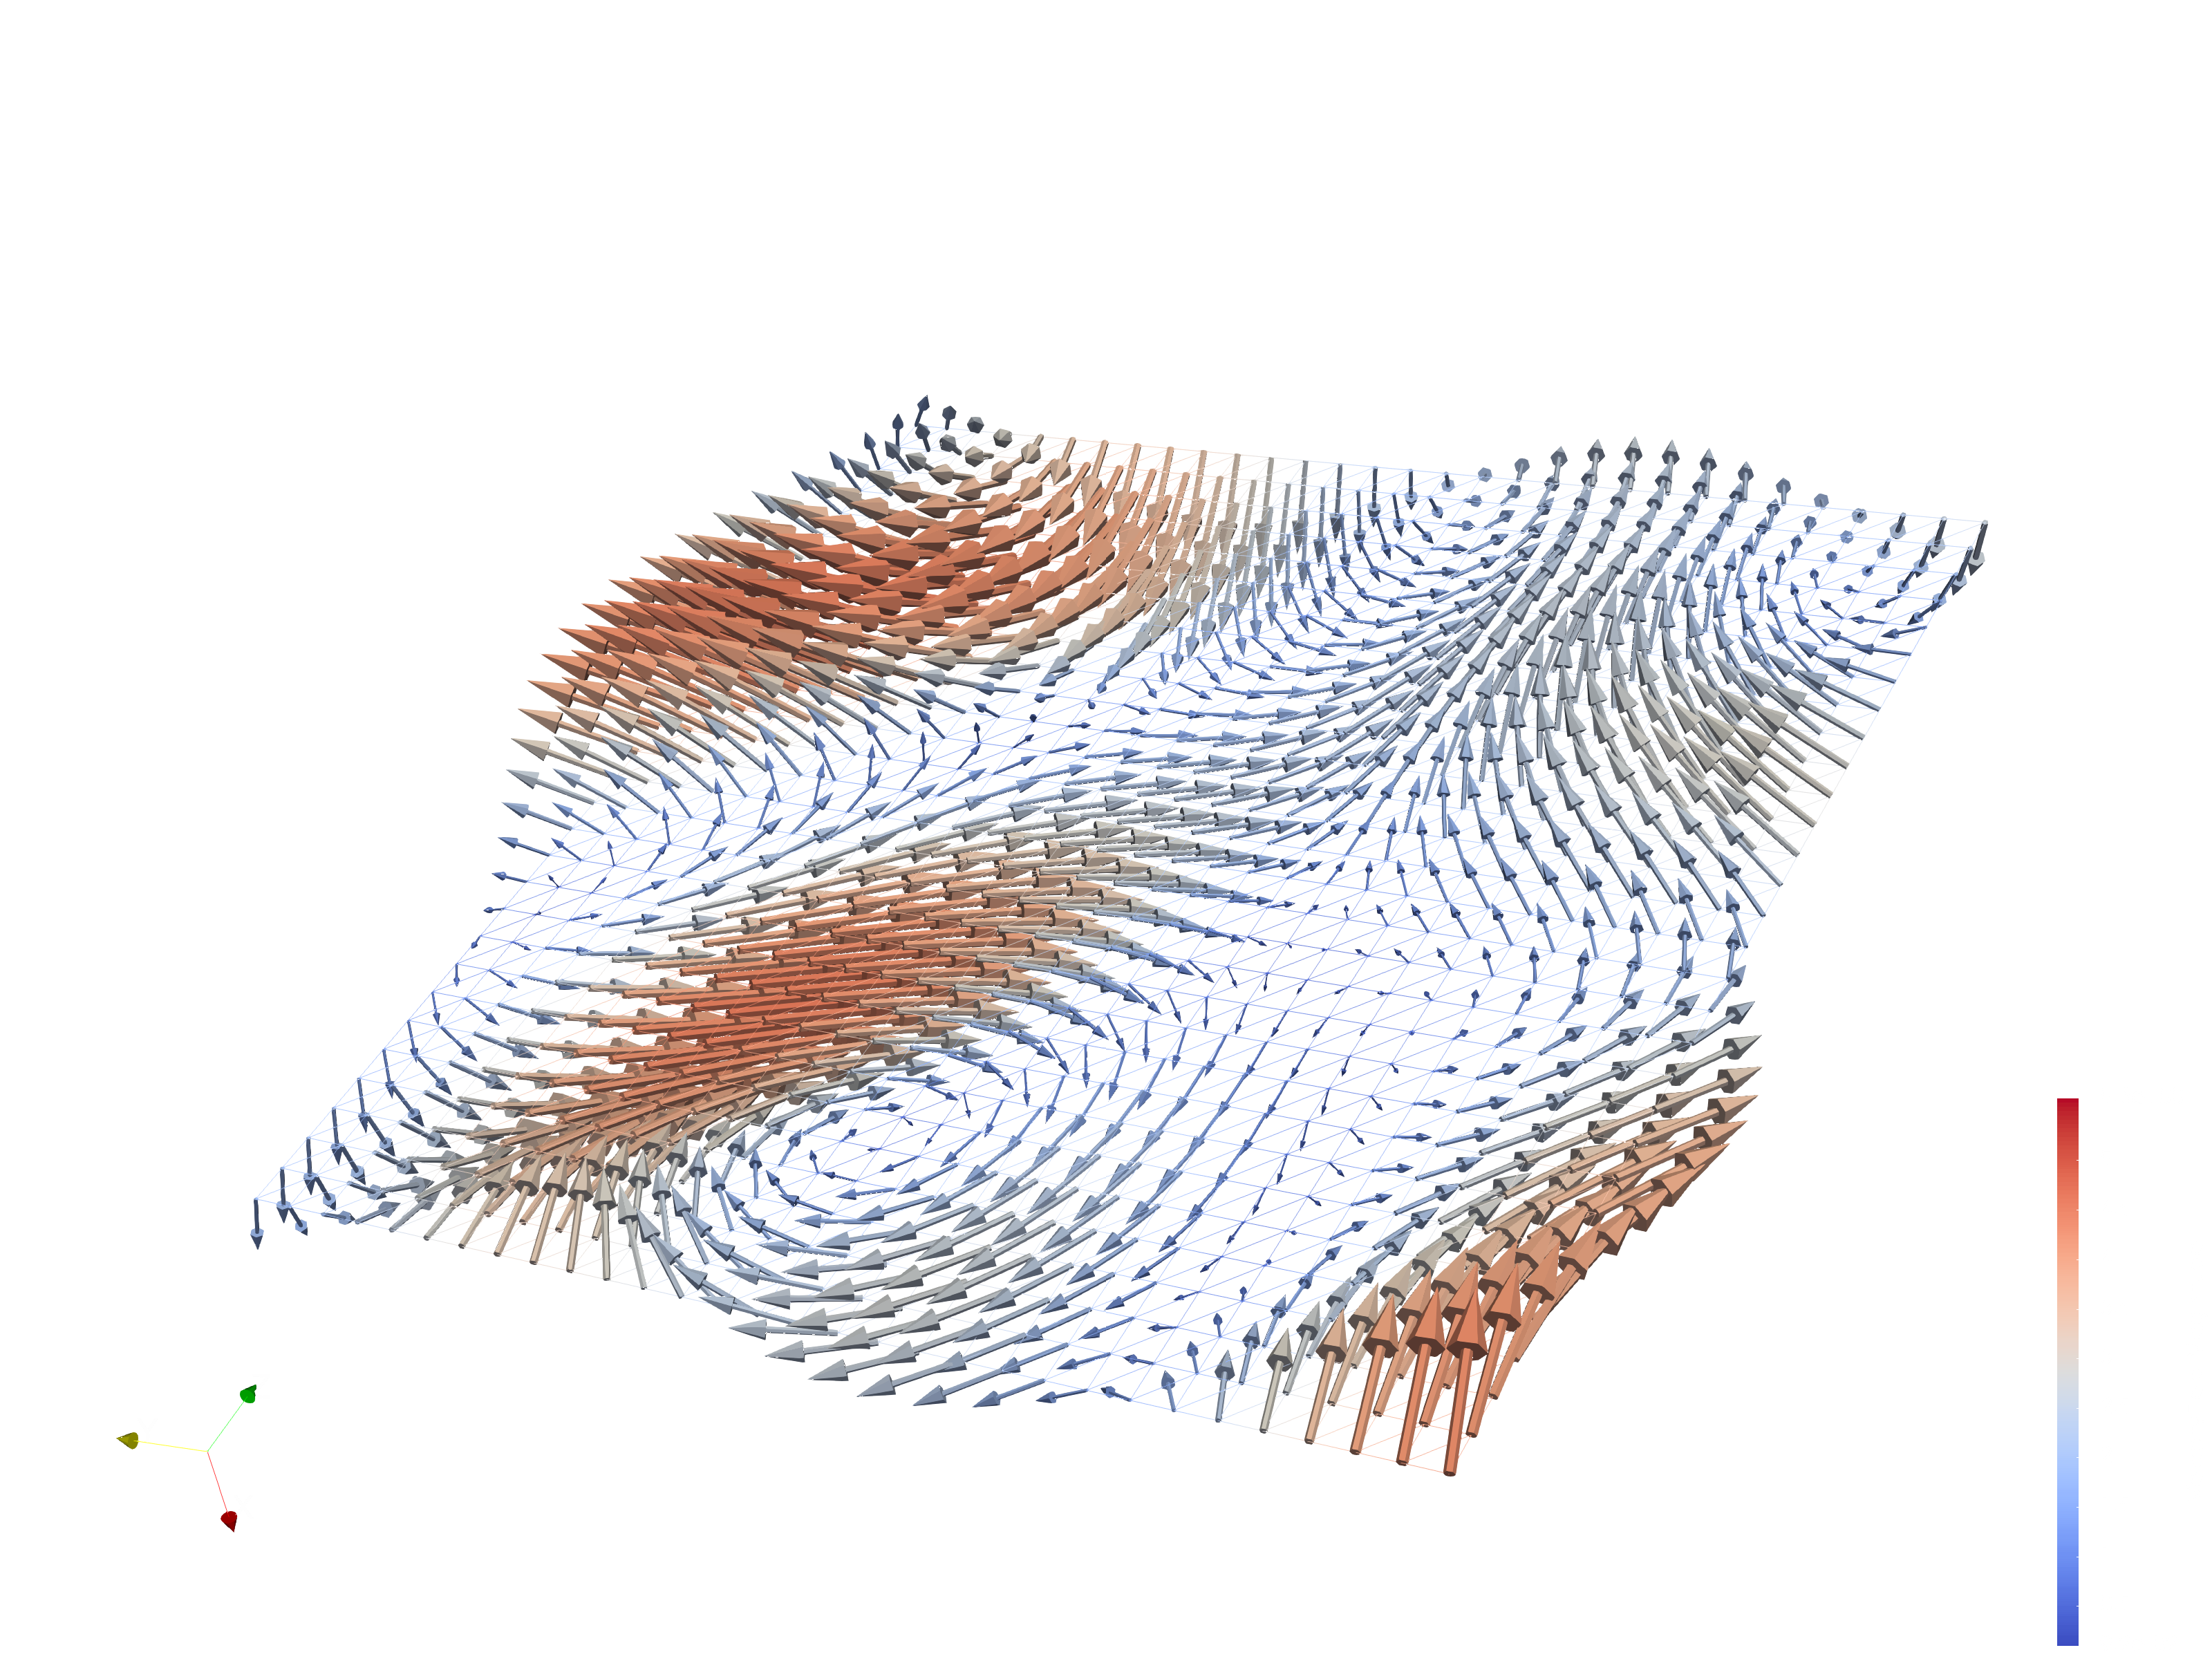
\includegraphics[width=0.4\linewidth]{images/spectral/spectral_n32_l10_f1000_k0pi3/spectral_x_normal_velocity_field_angle.png}}%
        \hfill       
        \subcaptionbox{плоскость $xy$, $z = 0$\label{img:spectral_slice_veloctiy_field_x_znormal_no_angle}} 
        {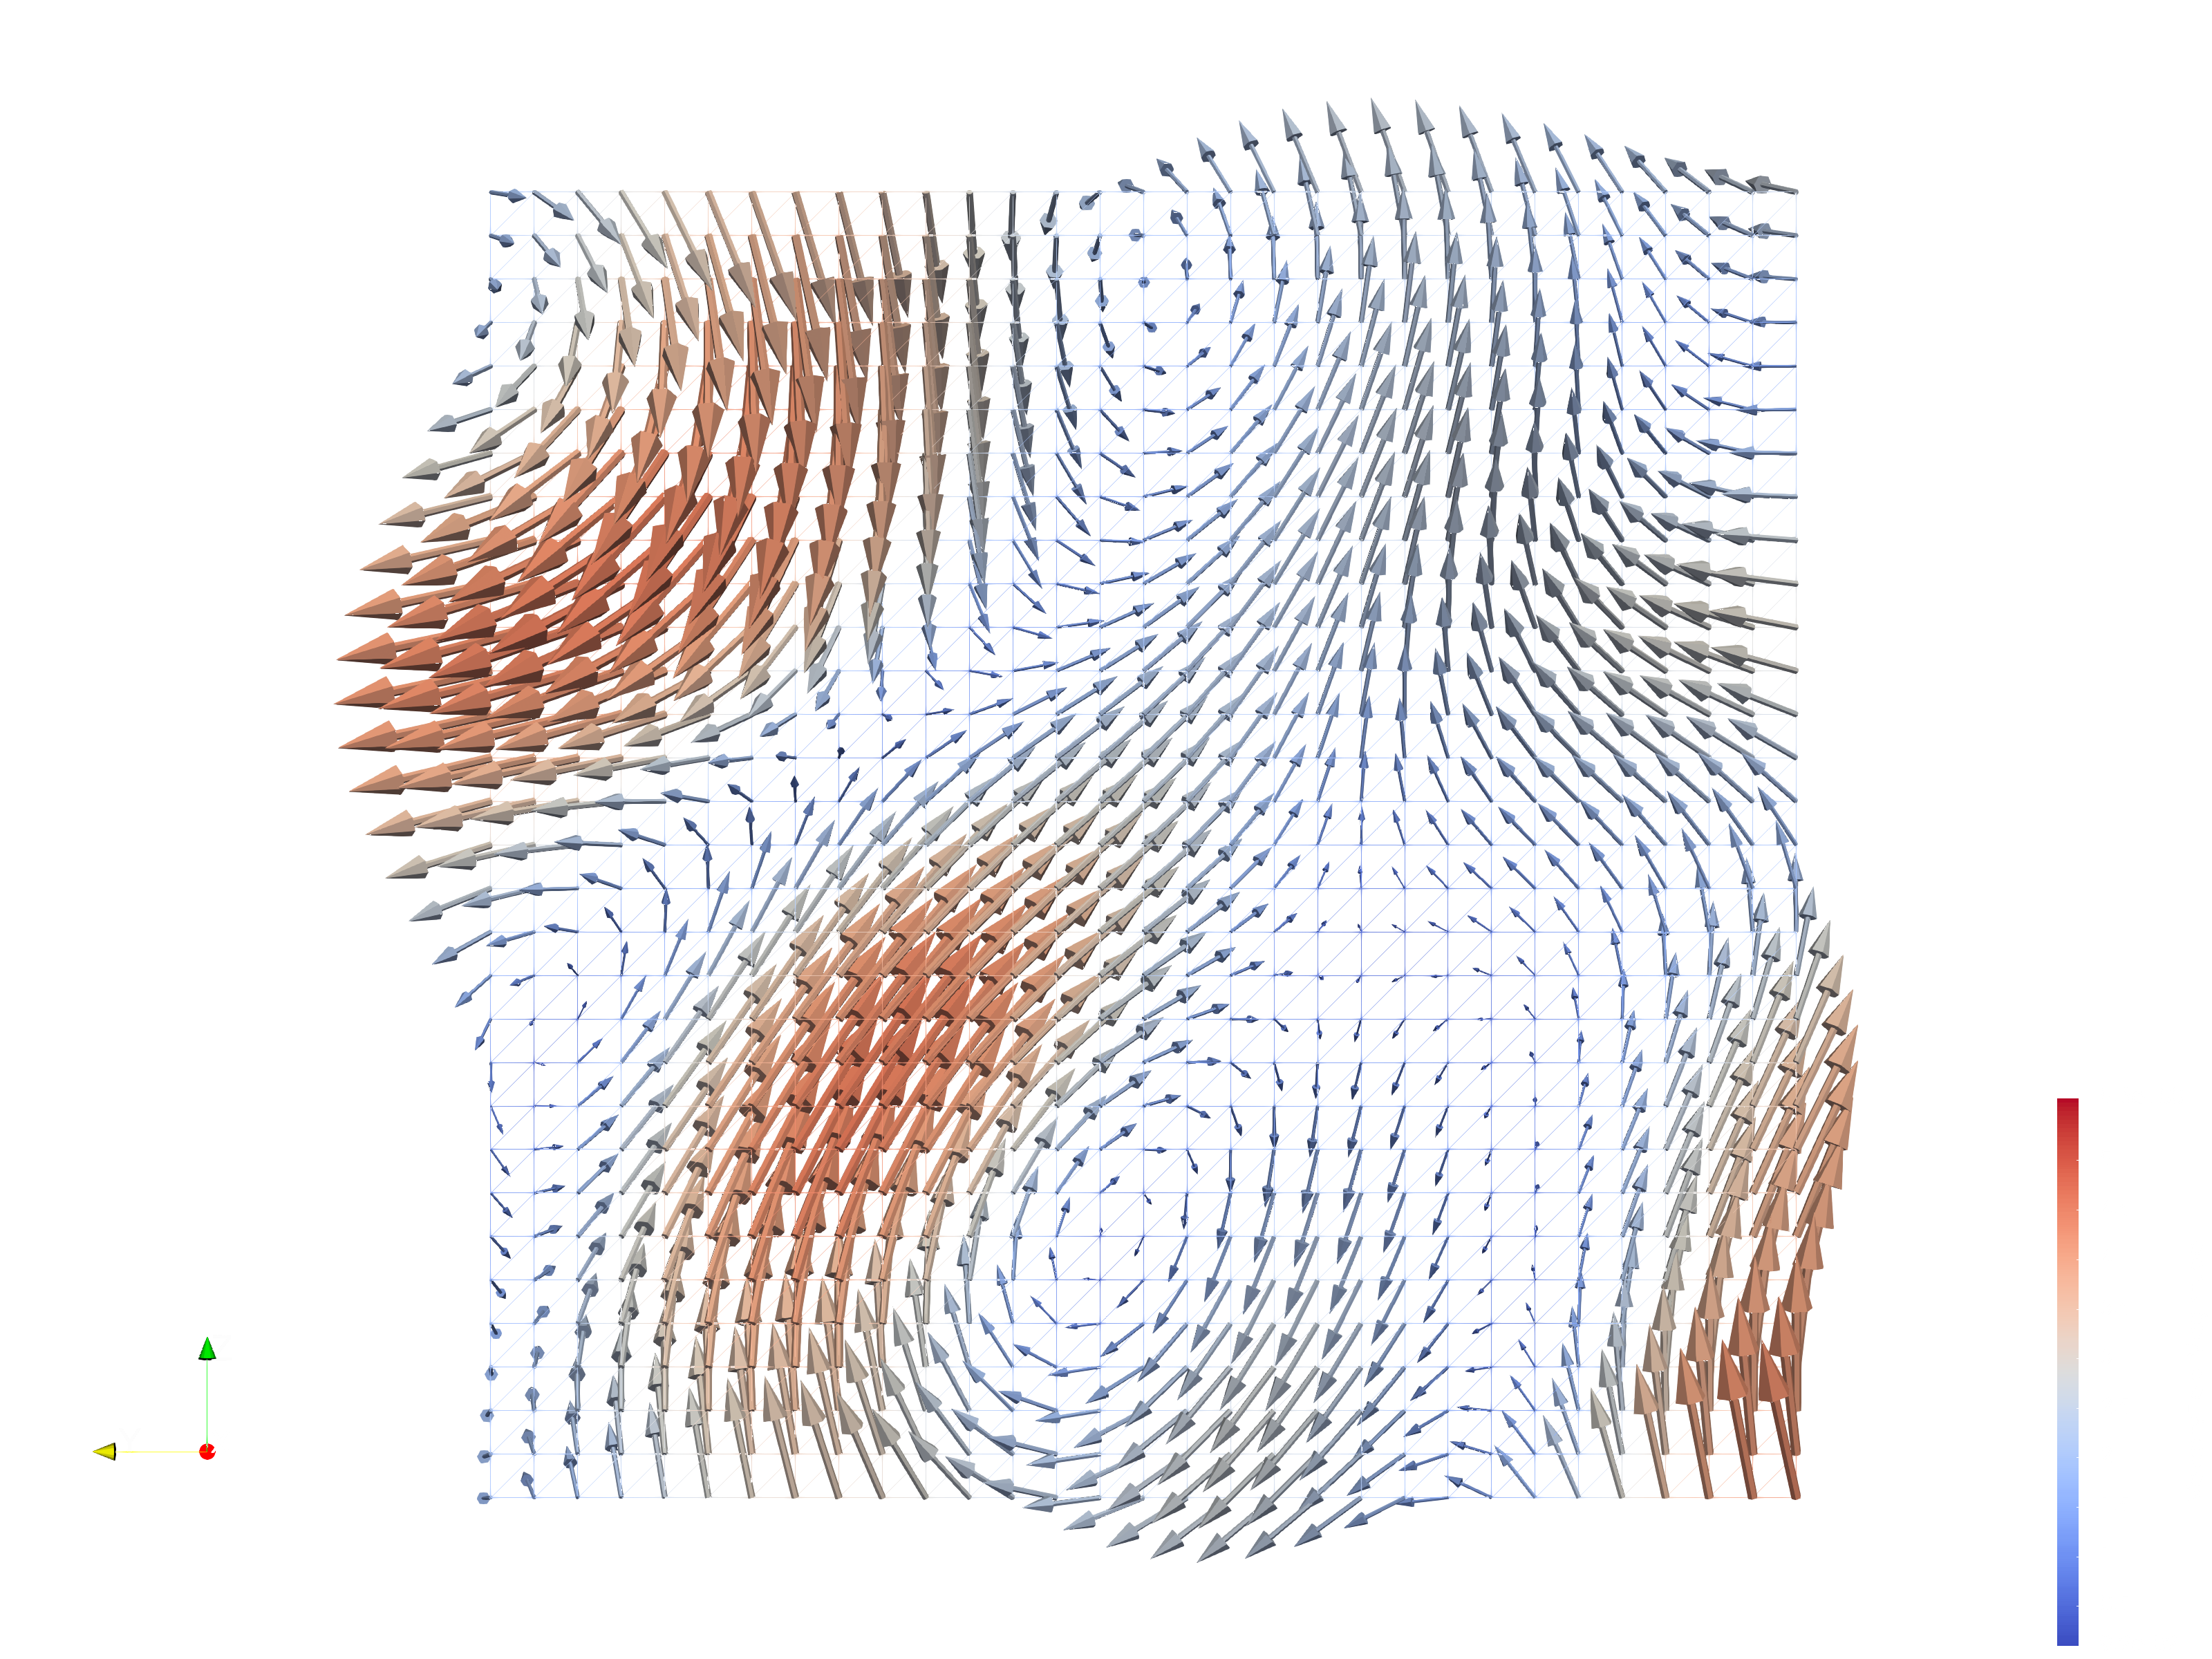
\includegraphics[width=0.4\linewidth]{images/spectral/spectral_n32_l10_f1000_k0pi3/spectral_x_normal_velocity_field.png}}
        \hfill
    }
    
    \onehalfspacing{Поле на картинке б представлено с линиями тока, расчитанными вдоль оси $y$}
    \caption{Поле флуктуаций сгенерированных трёхмерным стохастическим методом, цветом обозначена амплитуда флуктуаций}
    \label{img:velocity_fluctuation_field_for_spectral_1}  
\end{figure}

В отличие от стохастического метода, данный метод имеет явную зависимость вектора флуктуации от времени. Как говорилось выше, в данном случае распределение определяется сгенерированными частотами $\omega_0$. Мы можем выделить некоторый характерный период как $T = \frac{2 \pi}{\omega_0} = \frac{2 \pi}{k_0 v_0}$. Обычно при рассмотрении временных процессов берут период времени $100 T$, где $T = T_0$ -- характерный для задачи период (масштаб) времени. Шаг по времени выберем как $\Delta t = \frac{100 T_0}{N_{samples}}$ -- так мы можем трактовать поля сгенерированные во времени как одну реализацию поля флуктуаций. Ниже представлены сгенерированные поля для некоторых моментов времени. В общем случае, при данном шаге по времени наблюдается как плавный переход от одного поля к другому, так и достаточно резкий. Можно варьировать этот параметр путём задания среднеквадратичного отклонения для генерируемых частот -- $\omega_0$. Так для больших частот проявляется более частая смена ориентации векторов в пространстве.

%
%
% ТУТ КАРТИНКИ СГЕНЕРИРОВАННЫХ ПОЛЕЙ ВО ВРЕМЕНИ
%
%

На полученных реализациях мы можем оценить ковариационную функцию и последующими преобразованиями получить из неё и энергетический спектр. Ниже представлен рассчитанный на полученных реализациях тензор ковариаций относительно центра куба, совпадающего с началом координат, для различных направлений: по диагонали куба, по оси $x$, по оси $y$, по оси $z$, проходящие через начало координат. Различными цветами представлены компоненты тензора ковариаций. 

В случае однородной и изотропной турбулентности и несжимаемой жидкости есть возможность получить аналитическое выражение как для тензора ковариаций от функции энергетического спектра, так и для тензора спектра скорости от функции энергетического спектра \cite{Kraichnan70, pope2000turbulent}.

\begin{equation}
    \label{eq:part3_1}
    \left< \vec u (\vec x, t') \vec u (\vec x + \vec r, t) \right> = 2 D(t - t') \int_{0}^{\infty} E(k) \frac{\sin{(k r)}}{k r} dk 
\end{equation}

\begin{equation}
    \label{eq:part3_2}
    \Phi_{ij}(\vec k) = \frac{E(k)}{4 \pi k^2} \left( \delta_{ij} - \frac{k_i k_j}{k^2} \right)
\end{equation}

\noindent
здесь $k$ -- модуль волнового вектора, $k_i$ -- компонента волнового вектора.
Для обоих рассматриваемых методов генерация осуществляется в рамках однородной и изотропной турбулентности для несжимаемой жидкости, тем самым мы можем сравнить не только, например, спектральные характеристики, но и также провести сравнение других характеристик, таких как тензор ковариаций и тензора скоростей.

Рассмотрим полученные ковариационные функции на рассчитанные на 10000 реализаций поля флуктуаций с параметрами описанными выше.

\begin{figure}[!h]
    \center{
        \hfill
        \noindent \subcaptionbox[List-of-Figures entry]{диагональ куба\label{img:spectral_covariance_diagonal}} 
        {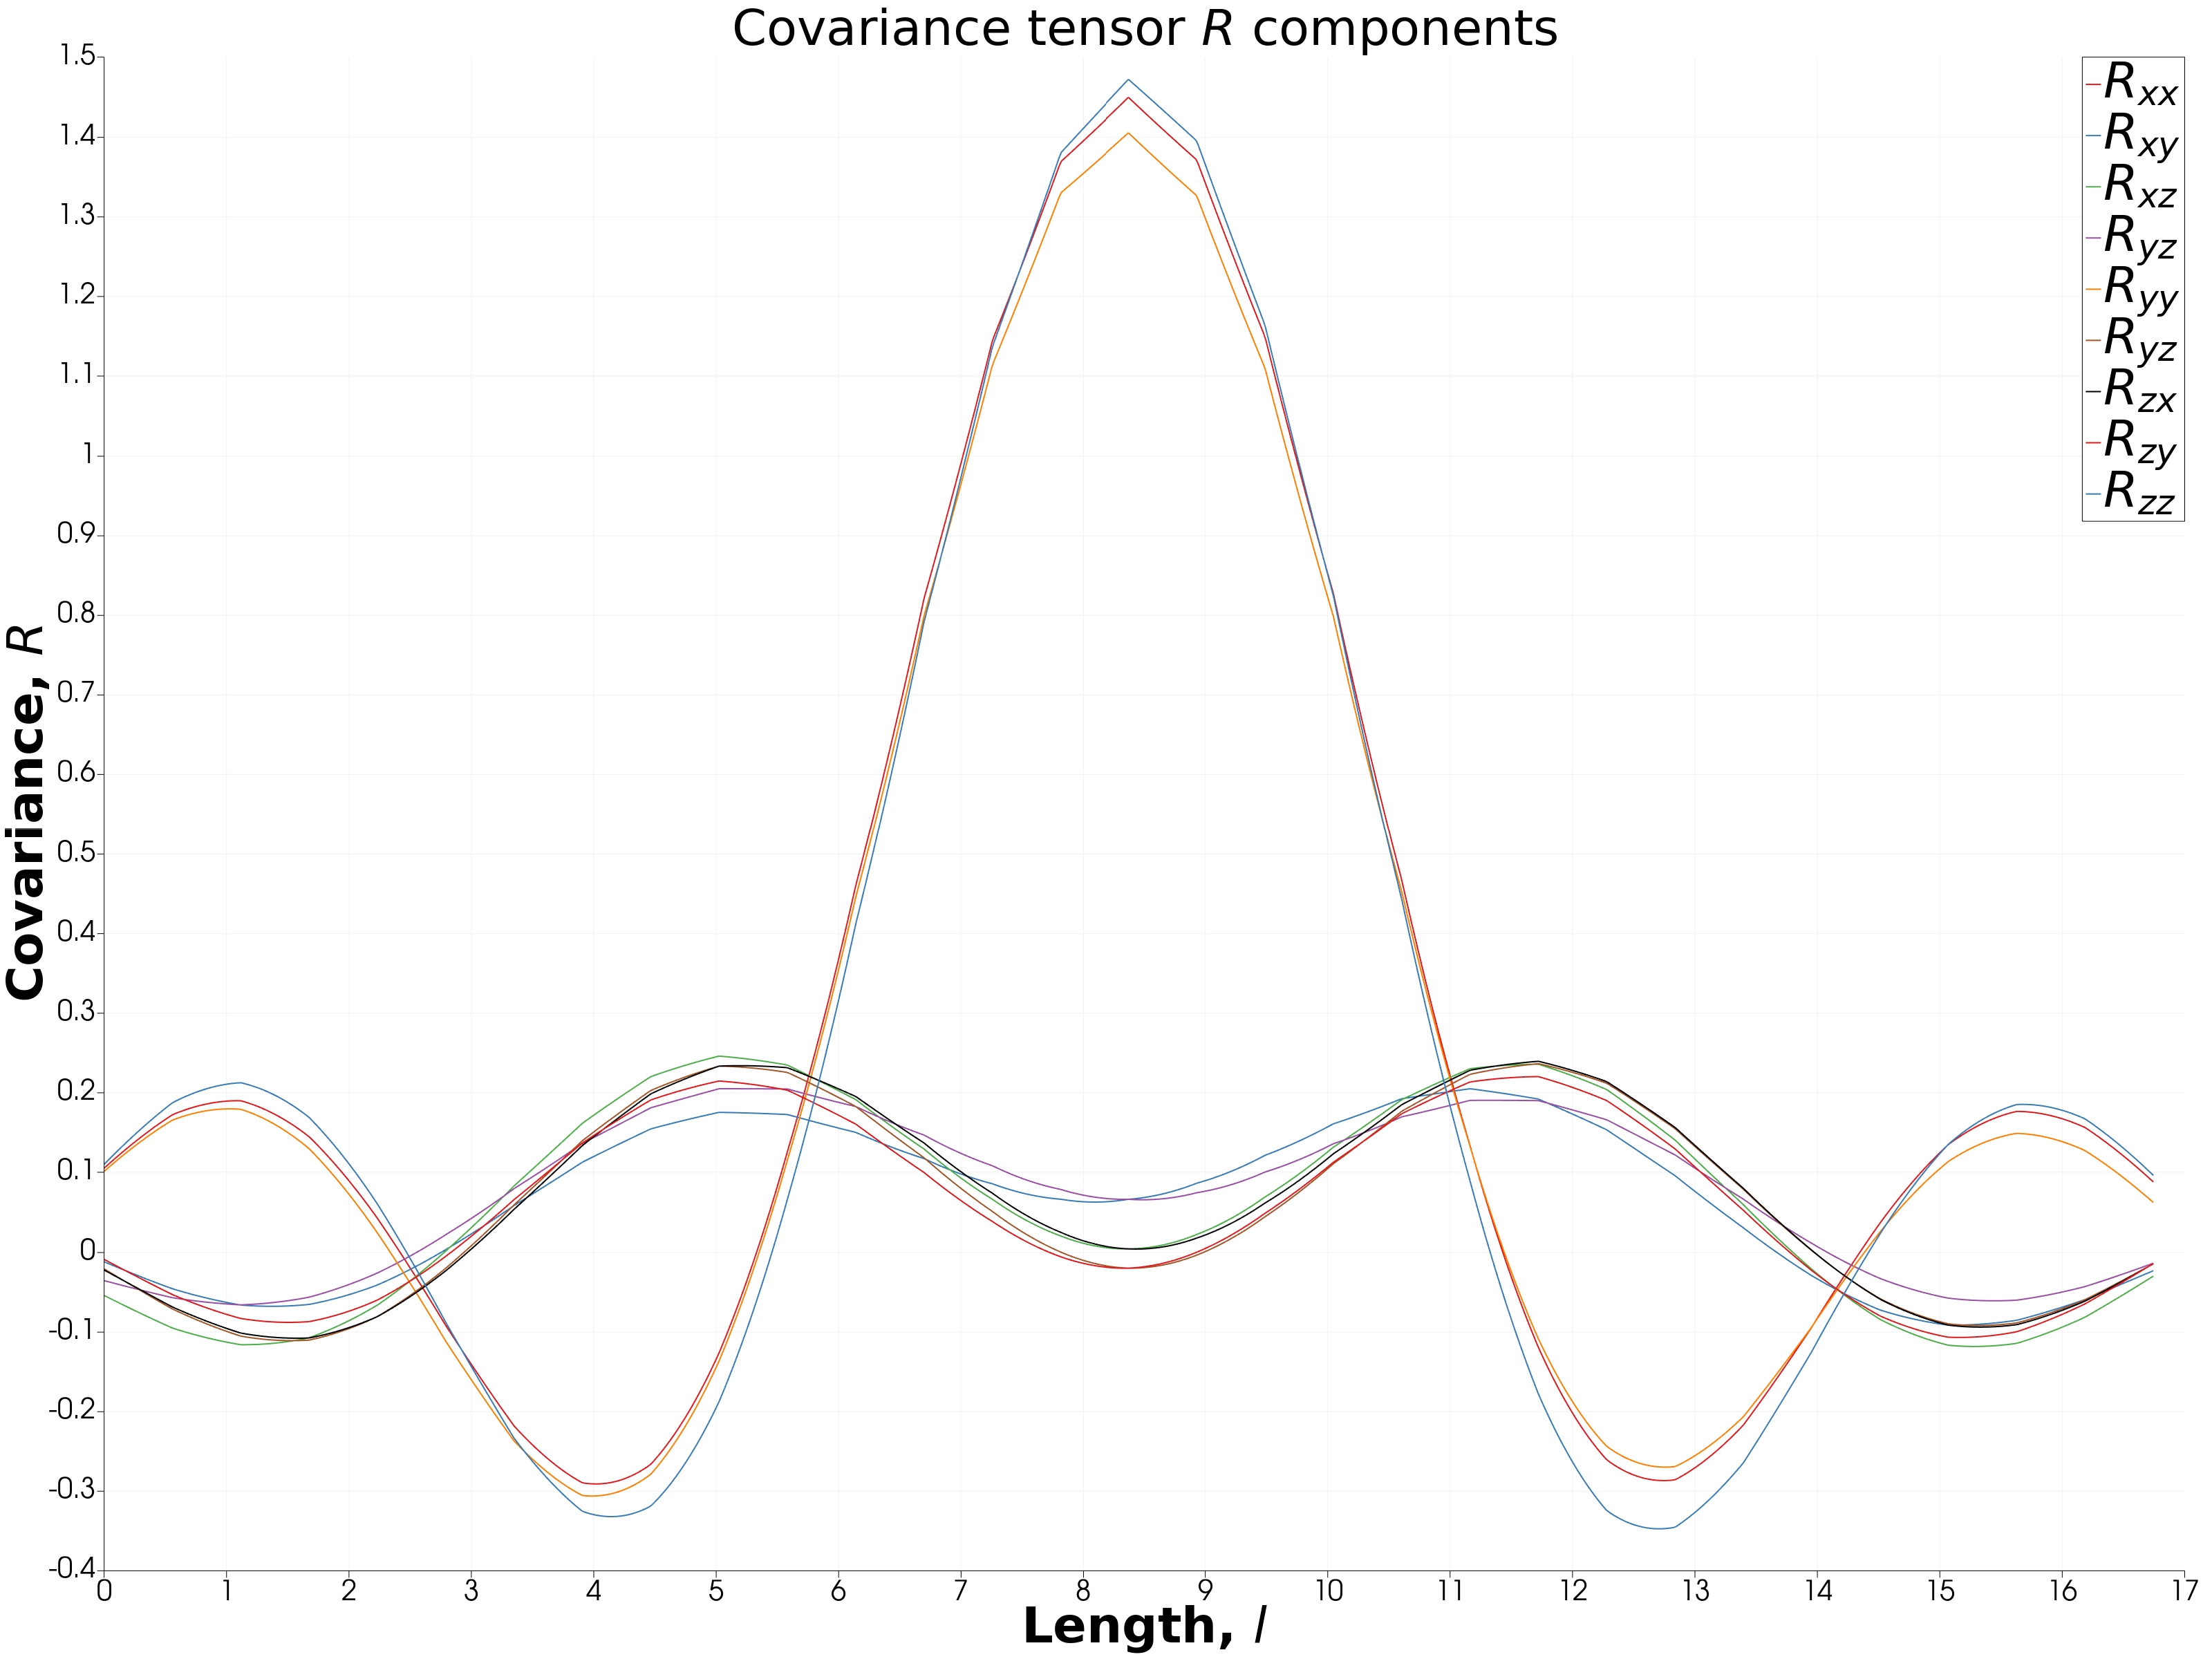
\includegraphics[width=0.4\linewidth]{images/spectral/spectral_n32_l10_f1000_k0pi3/covariance_function_diagonal.png}}%
        \hfill       
        \subcaptionbox{$x$\label{img:spectral_covariance_x}} 
        {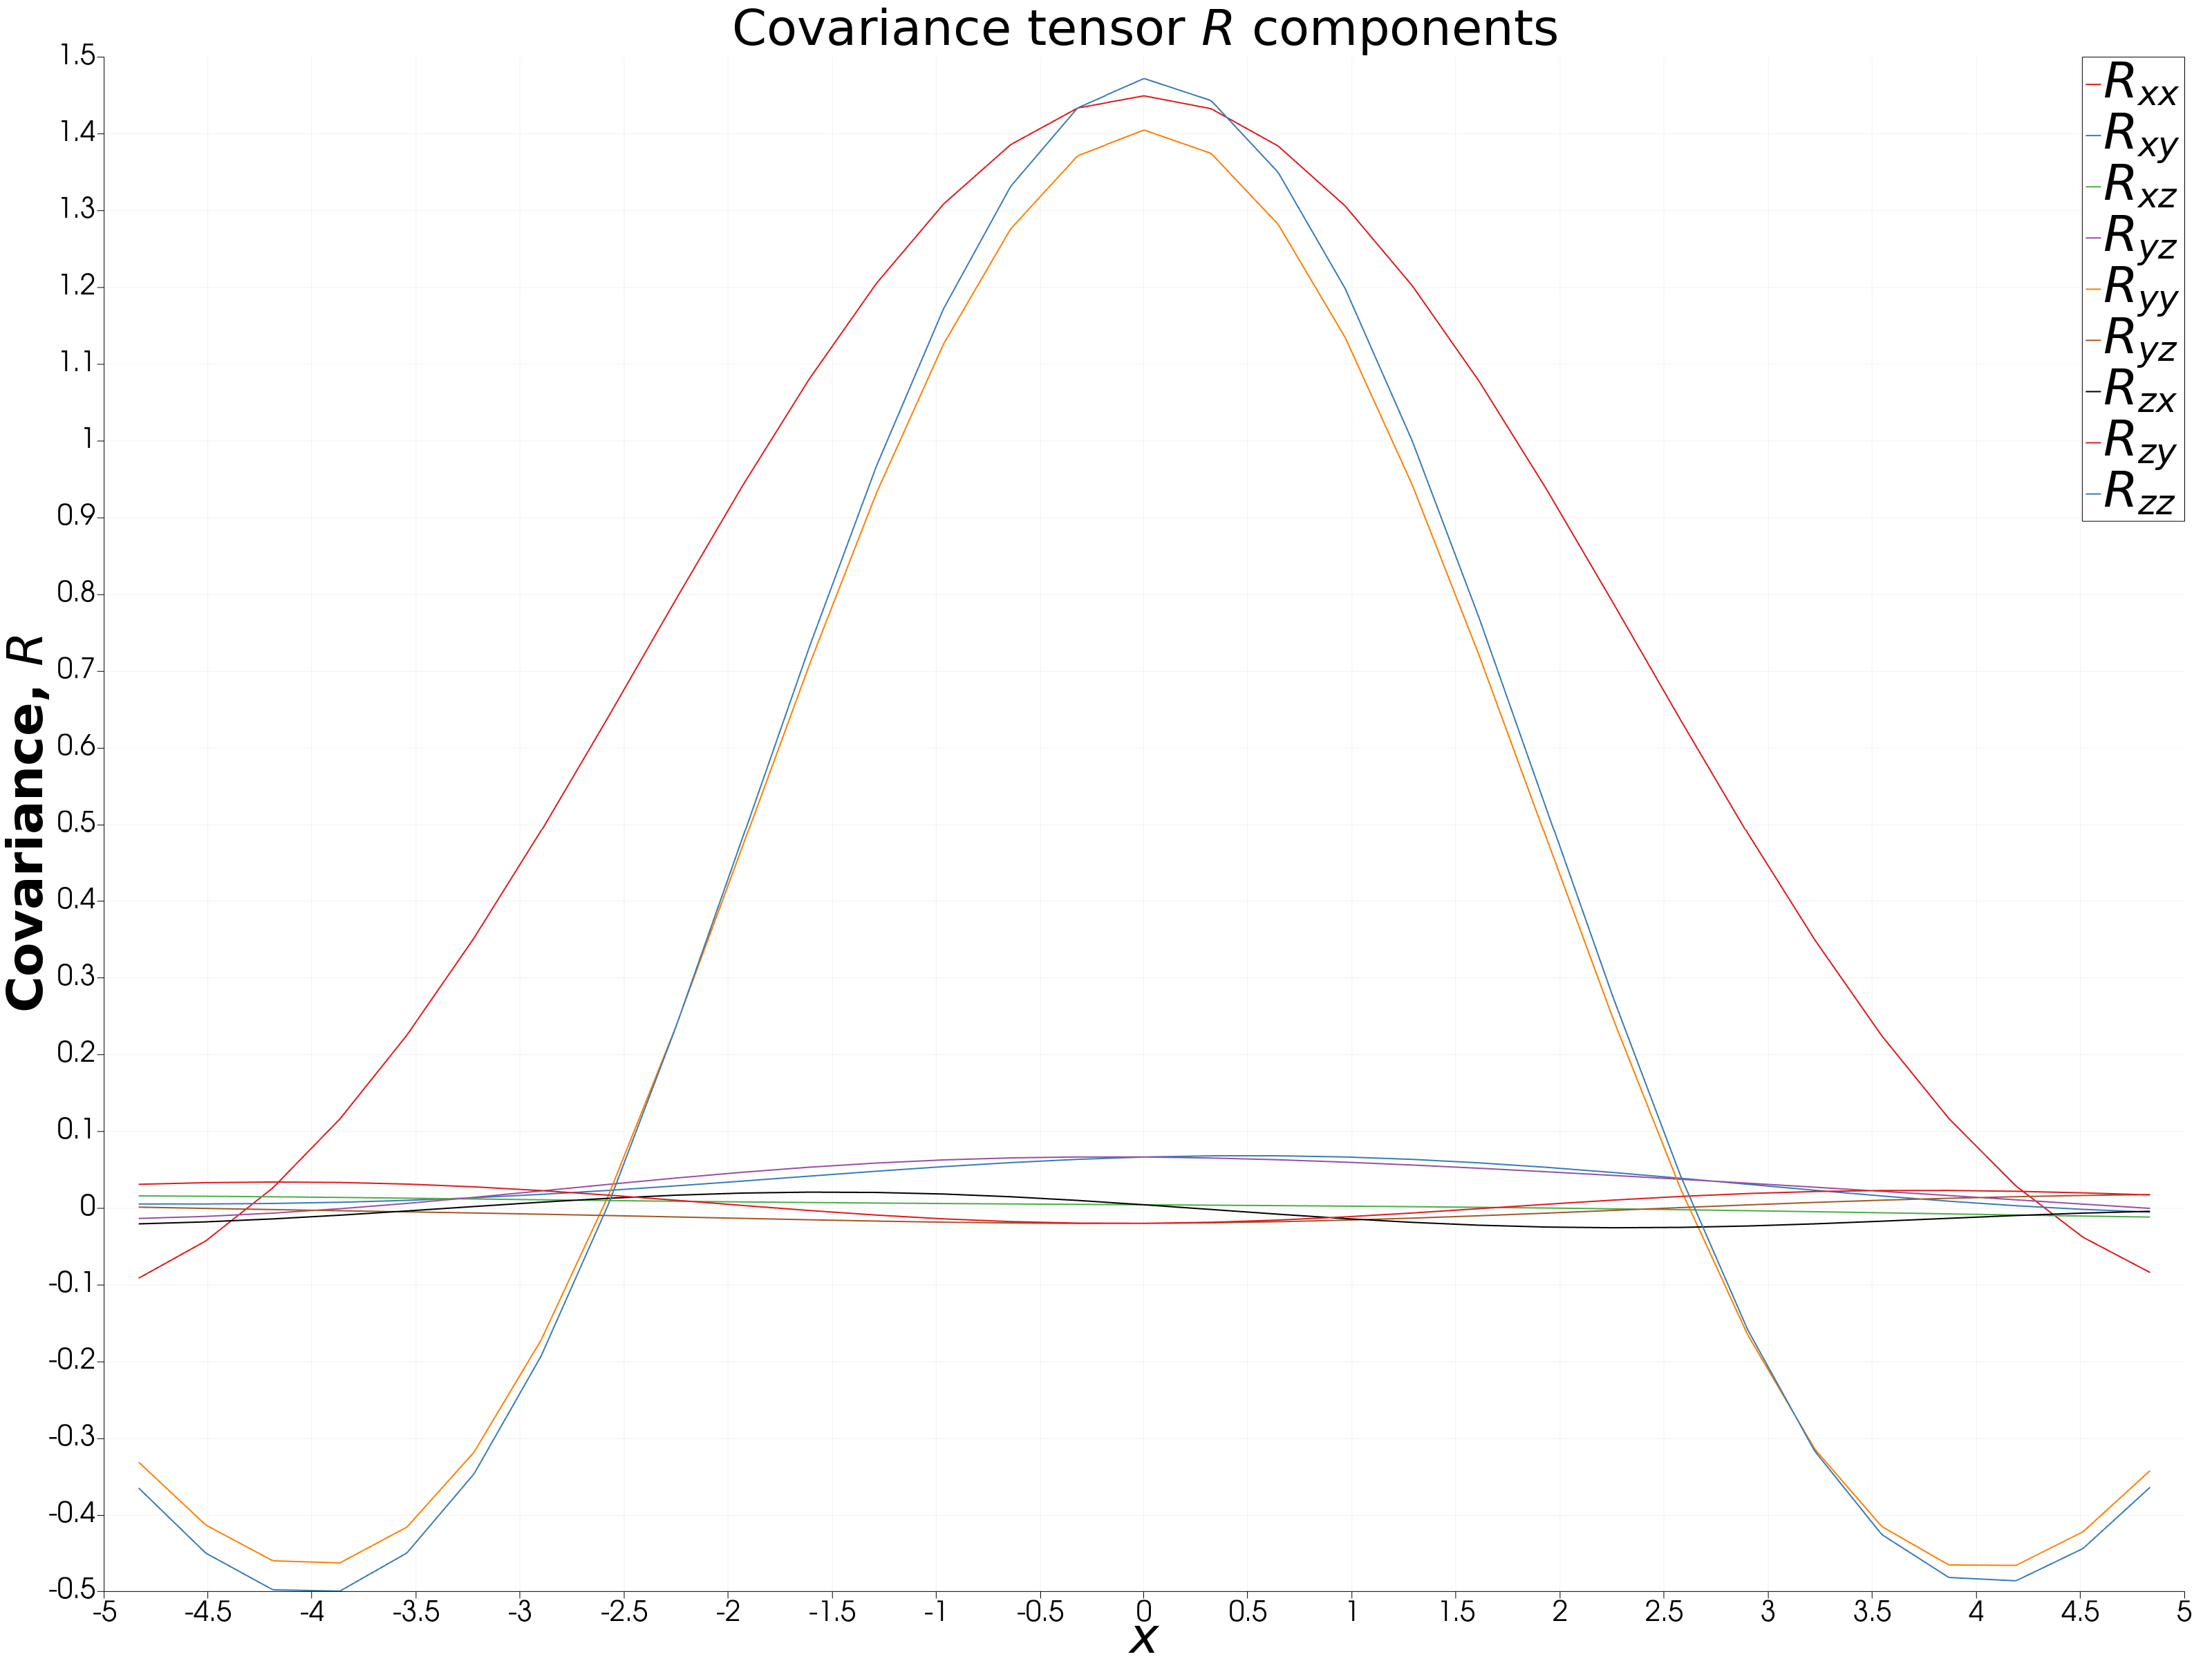
\includegraphics[width=0.4\linewidth]{images/spectral/spectral_n32_l10_f1000_k0pi3/covariance_function_x.png}} \\
        \hfill
        \subcaptionbox[List-of-Figures entry]{$y$\label{img:spectral_covariance_y}} 
        {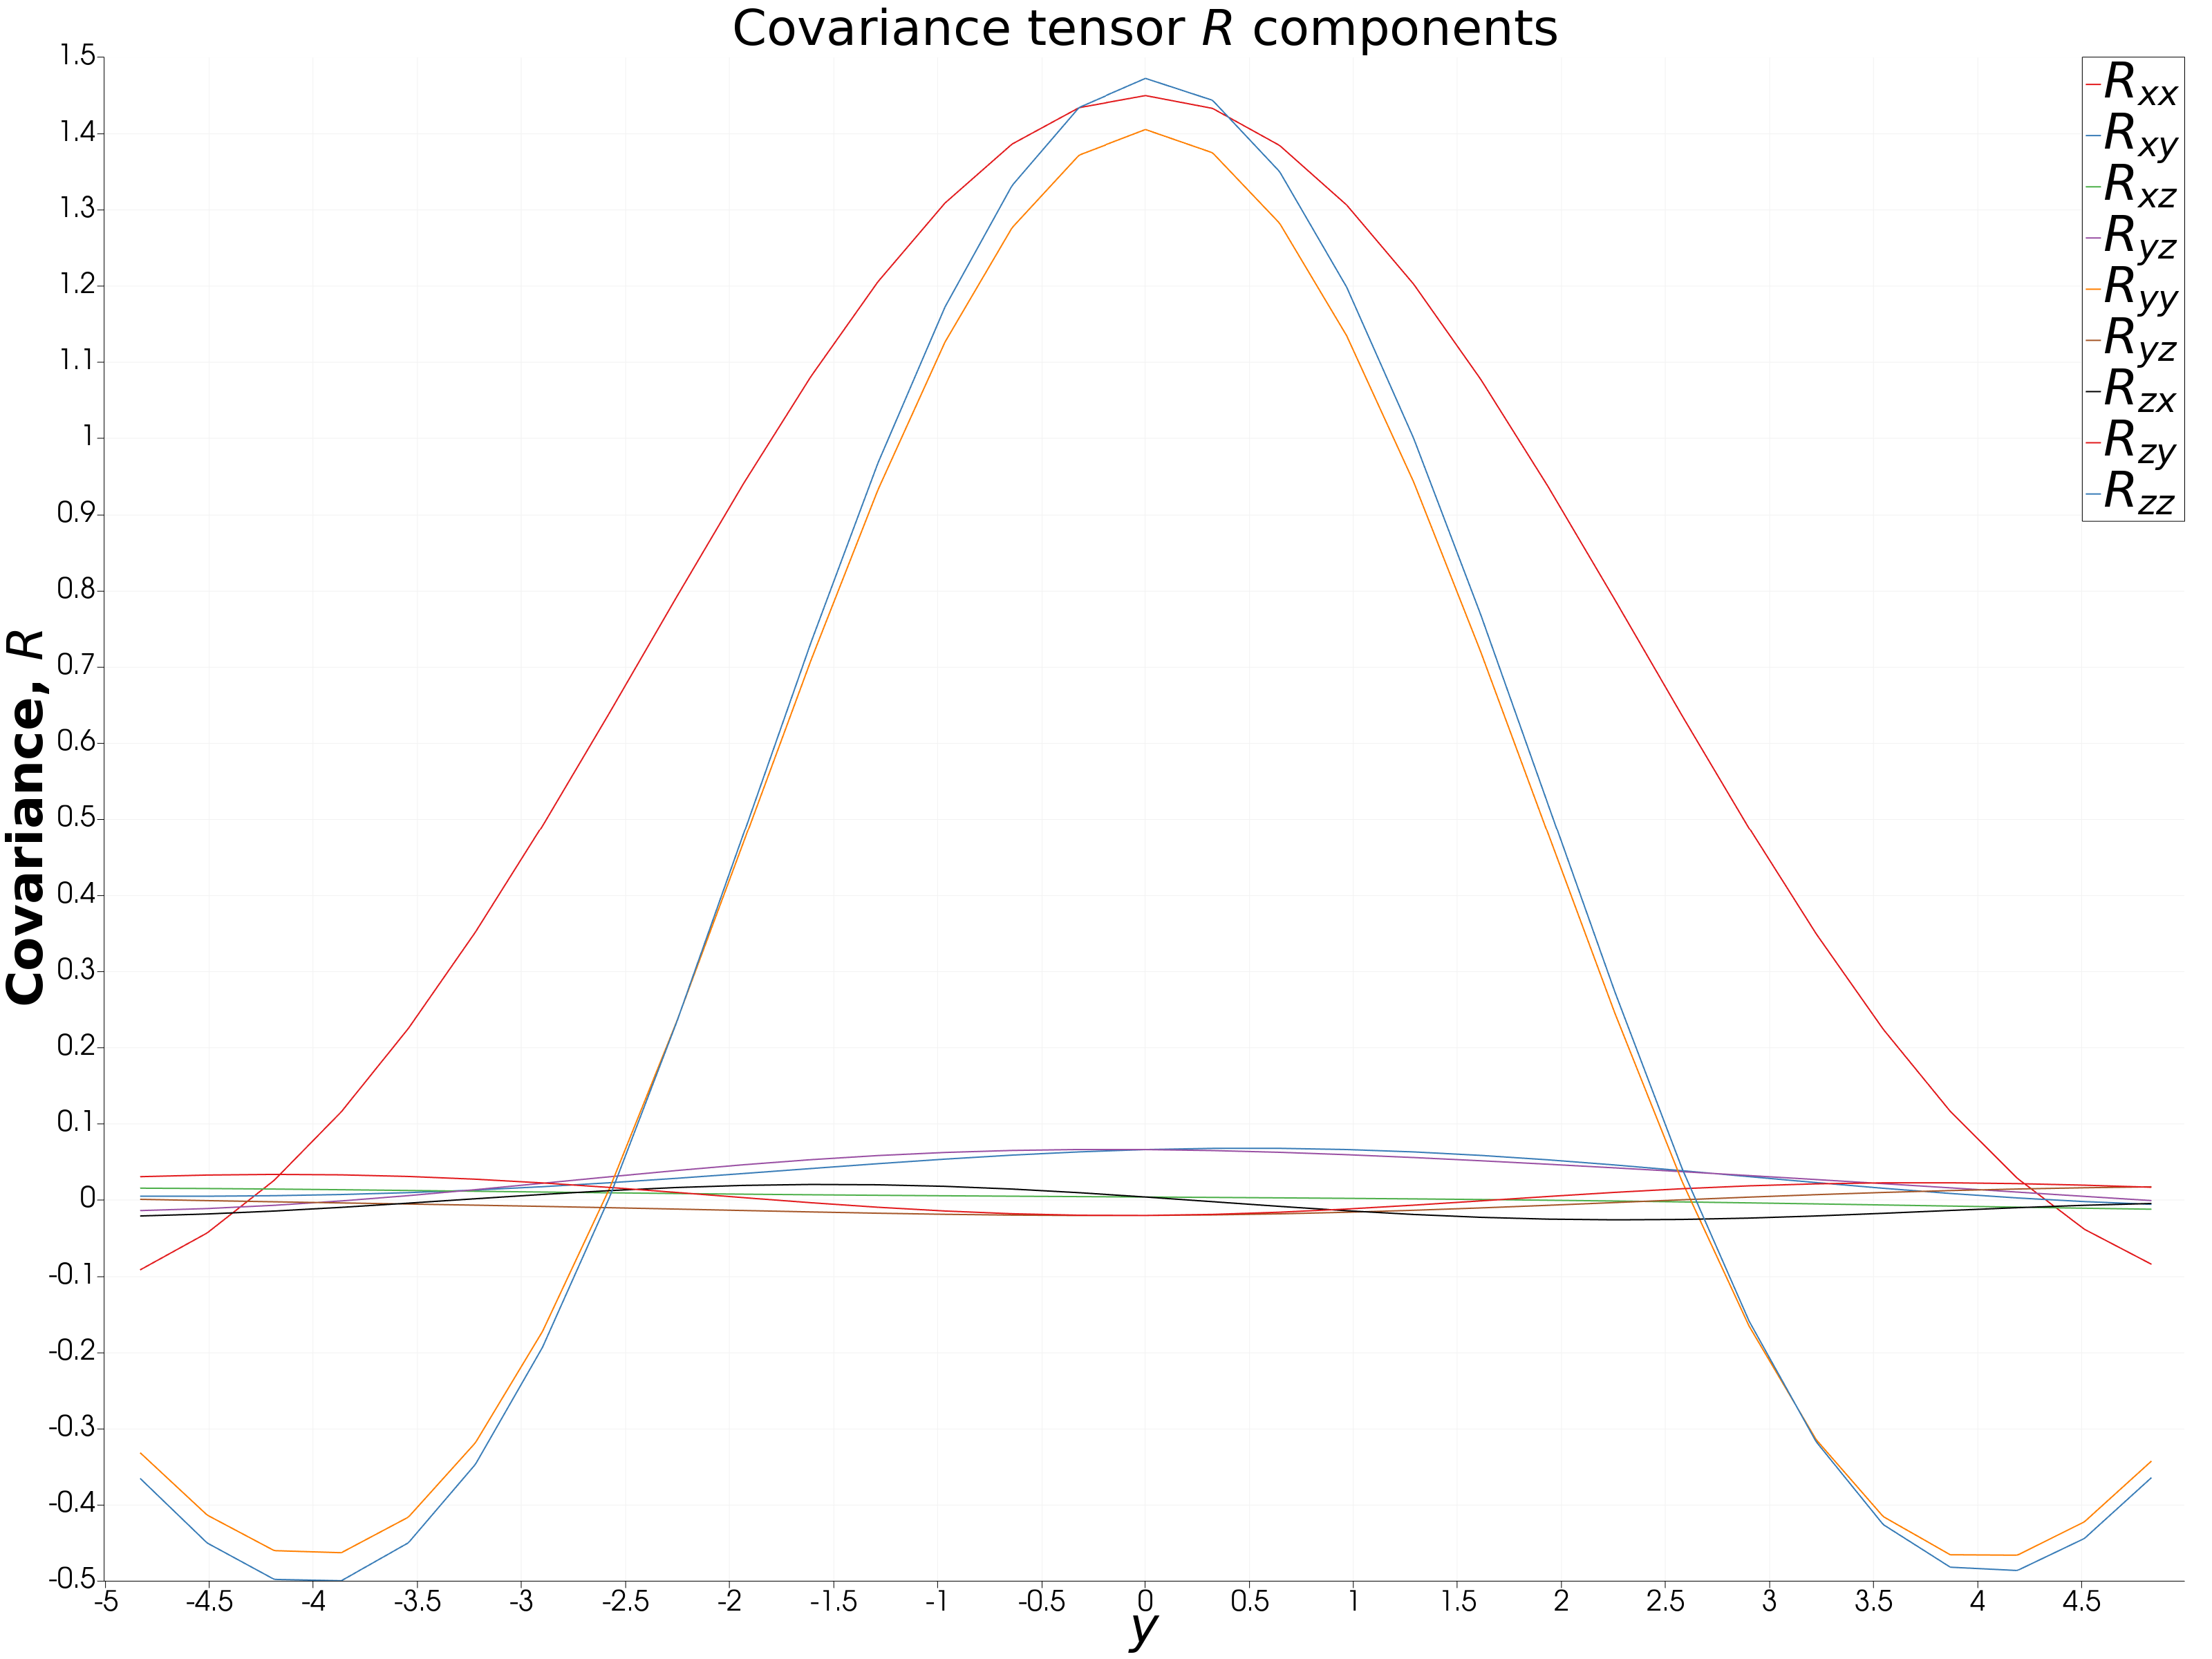
\includegraphics[width=0.4\linewidth]{images/spectral/spectral_n32_l10_f1000_k0pi3/covariance_function_y.png}}%
        \hfill       
        \subcaptionbox{$z$\label{img:spectral_covariance_z}} 
        {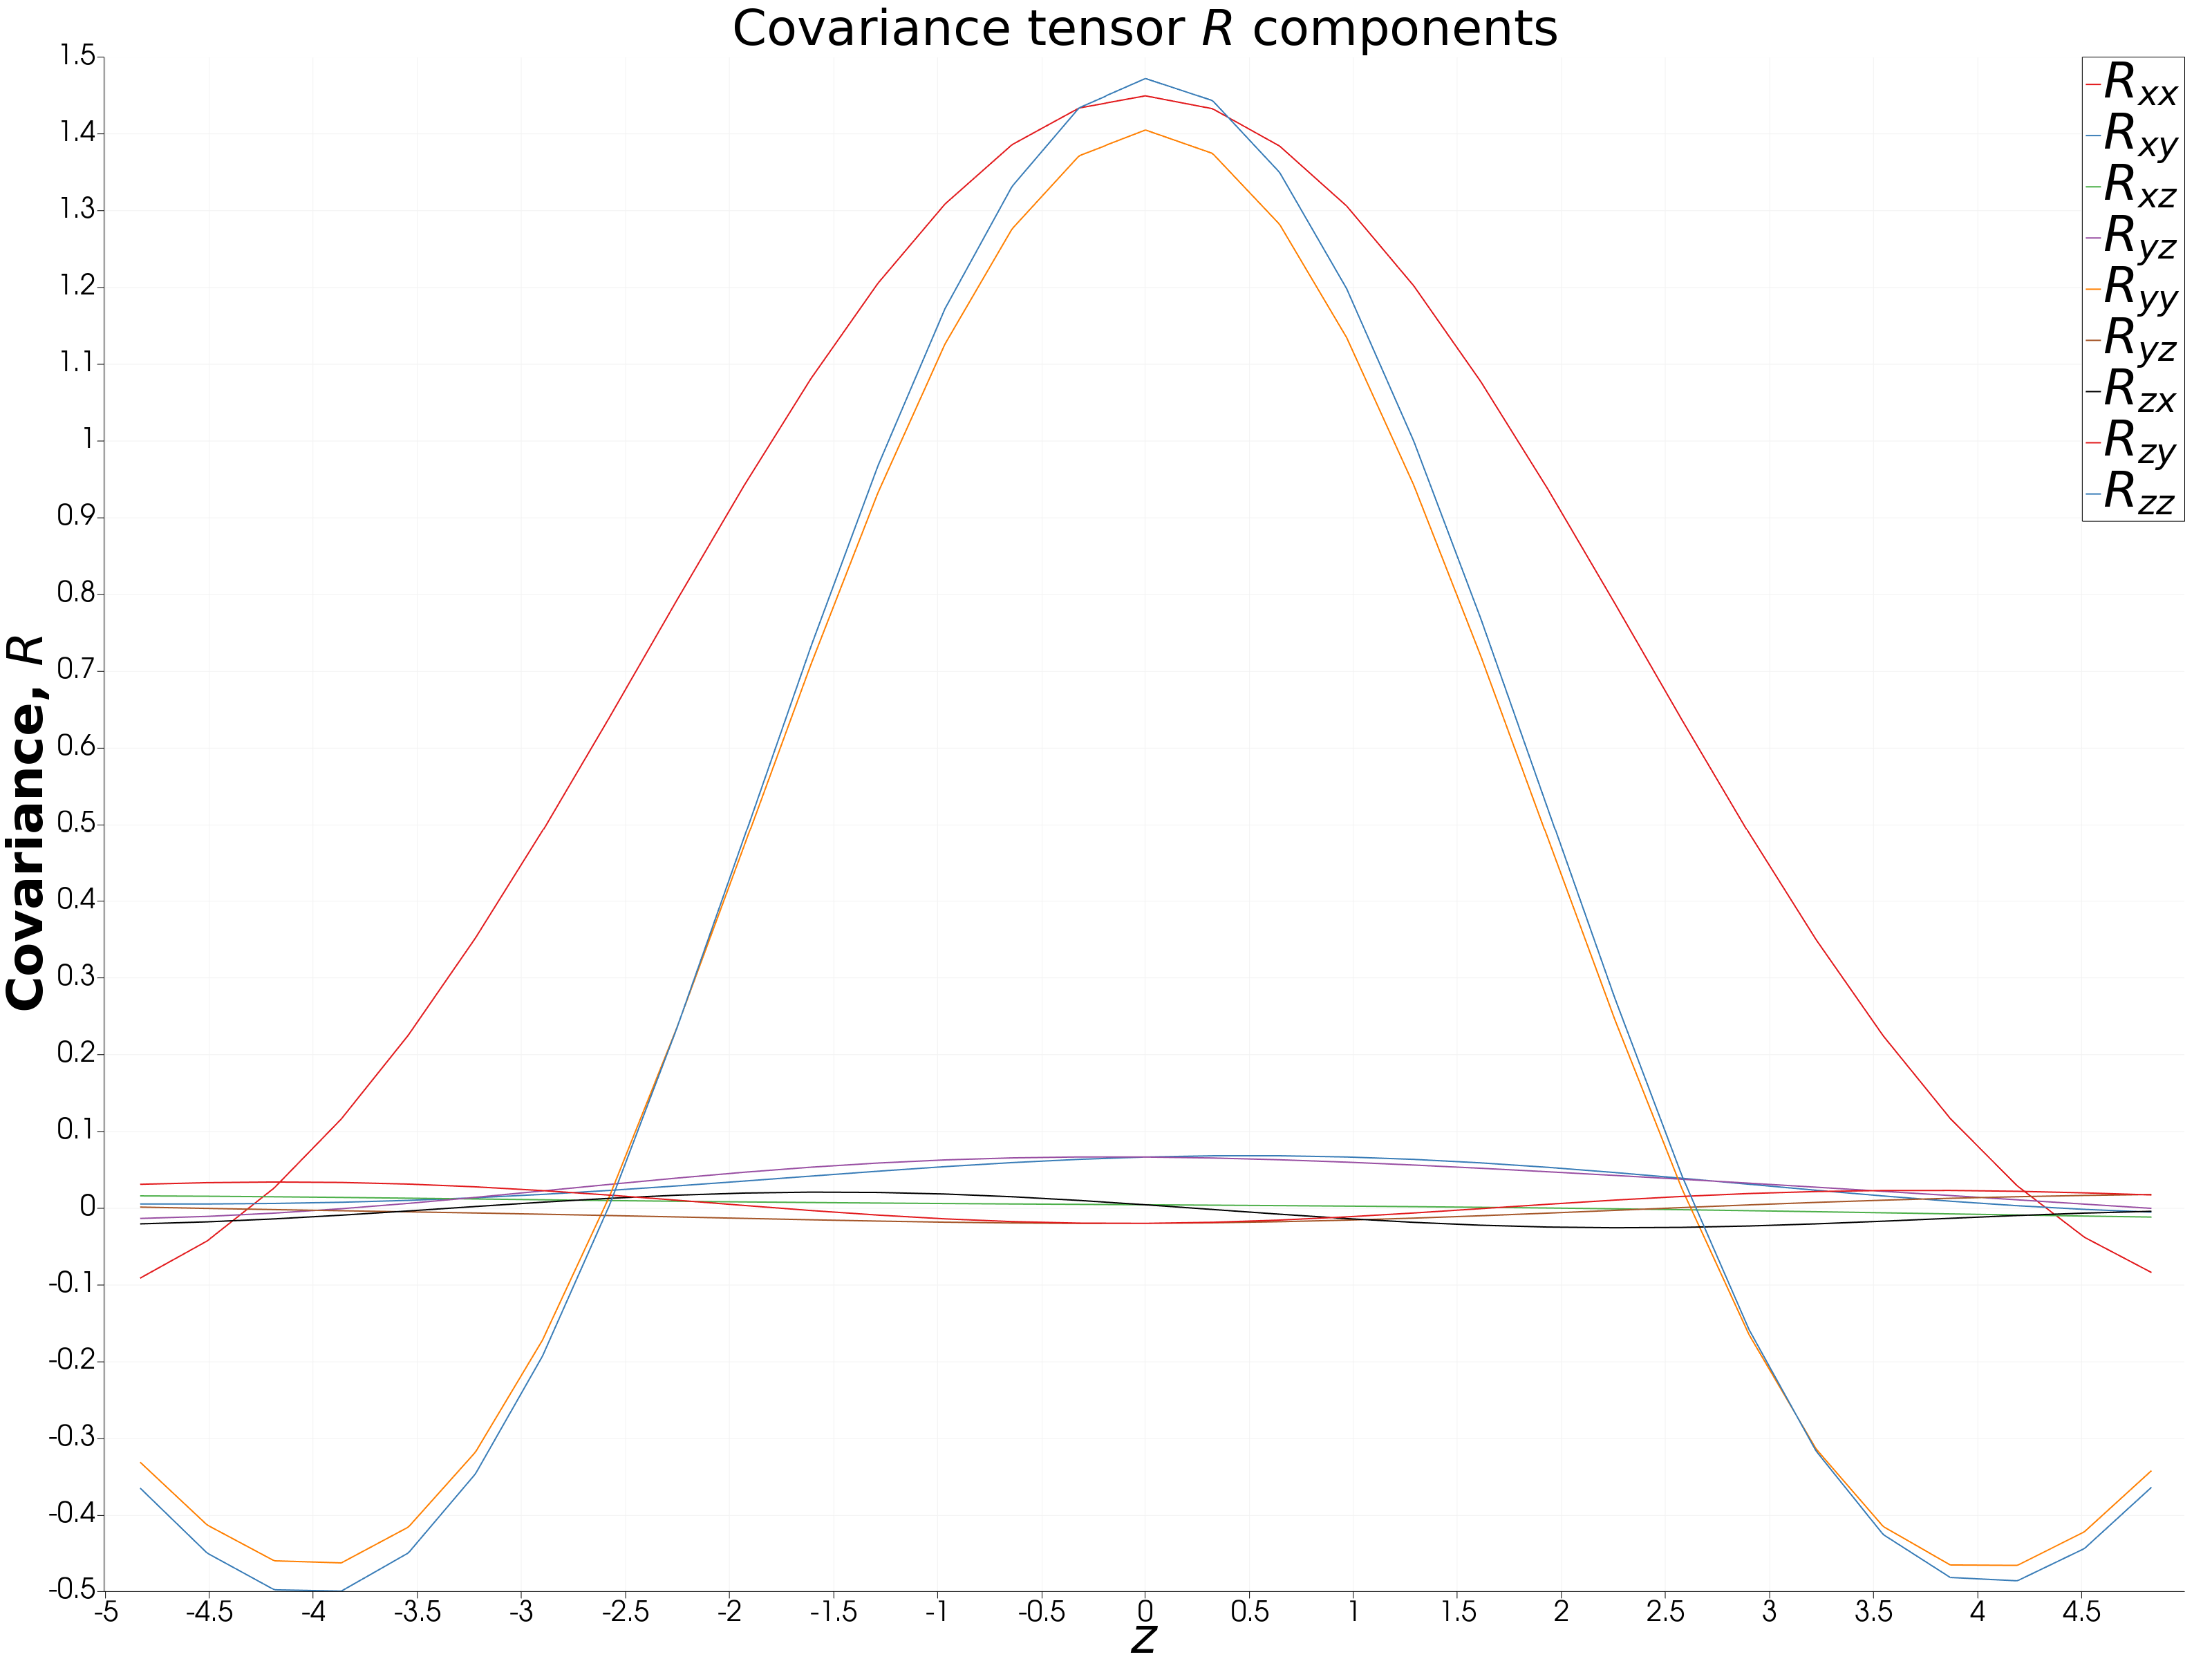
\includegraphics[width=0.4\linewidth]{images/spectral/spectral_n32_l10_f1000_k0pi3/covariance_function_z.png}}
        \hfill
    }
    
    \onehalfspacing{Поле на картинке б представлено с линиями тока, расчитанными вдоль оси $y$}
    \caption{Поле флуктуаций сгенерированных трёхмерным стохастическим методом, цветом обозначена амплитуда флуктуаций}
    \label{img:velocity_fluctuation_field_for_spectral_2}  
\end{figure}

По аналогии с методом Хуанга, мы можем генерировать поле флуктуаций как суперпозицию полей построенных для различных волновых чисел, а соответственно и для различных значений энергии. В этом случае $\vec u = \sum_{k_{i}} \vec u_i$, где $\vec u_i$ -- флуктуация, сгенерированная для определённого волнового числа $k_i$. Как и ранее, остается сложностью оценить наперед среднеквадратичное отклонение для проведения нормировки высоты спектральных линий для аппроксимации целевого спектра. Но мы можем сделать следующее, энергетический спектр турбулентности связан с кинетической энергии турбулентности $\kappa = \int_{0}^{\infty} E(k) dk$, отсюда мы можем взять, что $\kappa(k_m) = E(k_m) \Delta k$, и получаемую величину флуктуации скорости нормировать на значение $\sqrt{E(k_m) \Delta k}$. 

Одним из других подходов состоит в нормировке не результирующего значения флуктуации, а в нормировке амплитуд мод Фурье. В отличие от нормировки результирующего вектора флуктуаций, в данном подходе на выходе также получаются различные амплитуды флуктуаций с сохранением зависимости от амплитуды спектра. Для ускорения процесса генерации можно использовать разложение лишь по одной тригонометрической функции, например лишь по функции косинуса. В итоге можно использовать разложение представленное в виде:

\begin{equation}
    \label{eq:part3_3}
    \vec v(\vec r, t) = \alpha \sum_{n = 1}^{N} \vec p_n \cos( \vec k_n \cdot \vec r + \omega_n \cdot t + \psi)  
\end{equation}

\noindent 
здесь, $\vec p_n$ -- амплитуды мод Фурье, генерируемые изначально на единичной сфере так, чтобы $\vec p_n \cdot \vec k_n = 0$, для сохранения удовлетворению уравнению неразрывности, с последующим привидением к длине равной $\sqrt{E(k_n)\Delta k}$, $\psi_n$ - случайная фаза, добавленная для компенсации исключения нечетных мод, генерируемая например из равномерного распределения в пределах $-\pi$ до $\pi$, $\alpha$ -- нормировочный коэффициент, который можно взять, например $\sqrt{\frac{2}{N}}$, как в методе Смирнова(\ref{sect2_2}), либо провести нормировки на кинетическую энергию по аналогии с методом Шура (\ref{sect2_4}): $\sqrt{\frac{1}{\sum_{n=1}^{N} E(k_n) \Delta k_n}}$. По построению амплитуд Фурье лучше всего использовать последнее определение для нормировочного коэффициента $\alpha = \sqrt{\frac{\beta}{\sum_{n=1}^{N} E(k_n) \Delta k_n}}$, после проведения тестовых расчётов мы получили что оптимальным значение для коэффициента $\beta \approx 2$. Связано это с тем, чтобы в формуле \eqref{eq:kriging_equation15} компенсировать коэффициент $\frac{1}{2}$

Для проведения статистического анализа предлагаемой модификации спектрального метода использовалось 5000 реализаций со следующими параметрами:
\begin{enumerate}
    \item Длина куба: $l = 10$, центр совпадает с началом координат;
    \item Число разбиений по каждой из сторон куба: $n = 51$;
    \item Число взятых мод Фурьe: $N = 1000$;
    \item Интервал волновых чисел: $(k_{min} = 0.01, k_{max} = 10$, число разбиений для дискретизации спектра совпадает с числом мод Фурье;
\end{enumerate}

Наименьшее волновое число для рассматриваемой сетке: $k_{min} = \frac{2 \pi}{l} \approx 0.6283$ -- максимальное волновое число: $k_{max} = \frac{\pi}{\dfrac{l}{n}} \approx 16.022$. Приведём сравнение спектра рассчитанного для приведённого выше числа сгенерированных реализаций с входным спектром.

\begin{figure}[ht] 
    \center
    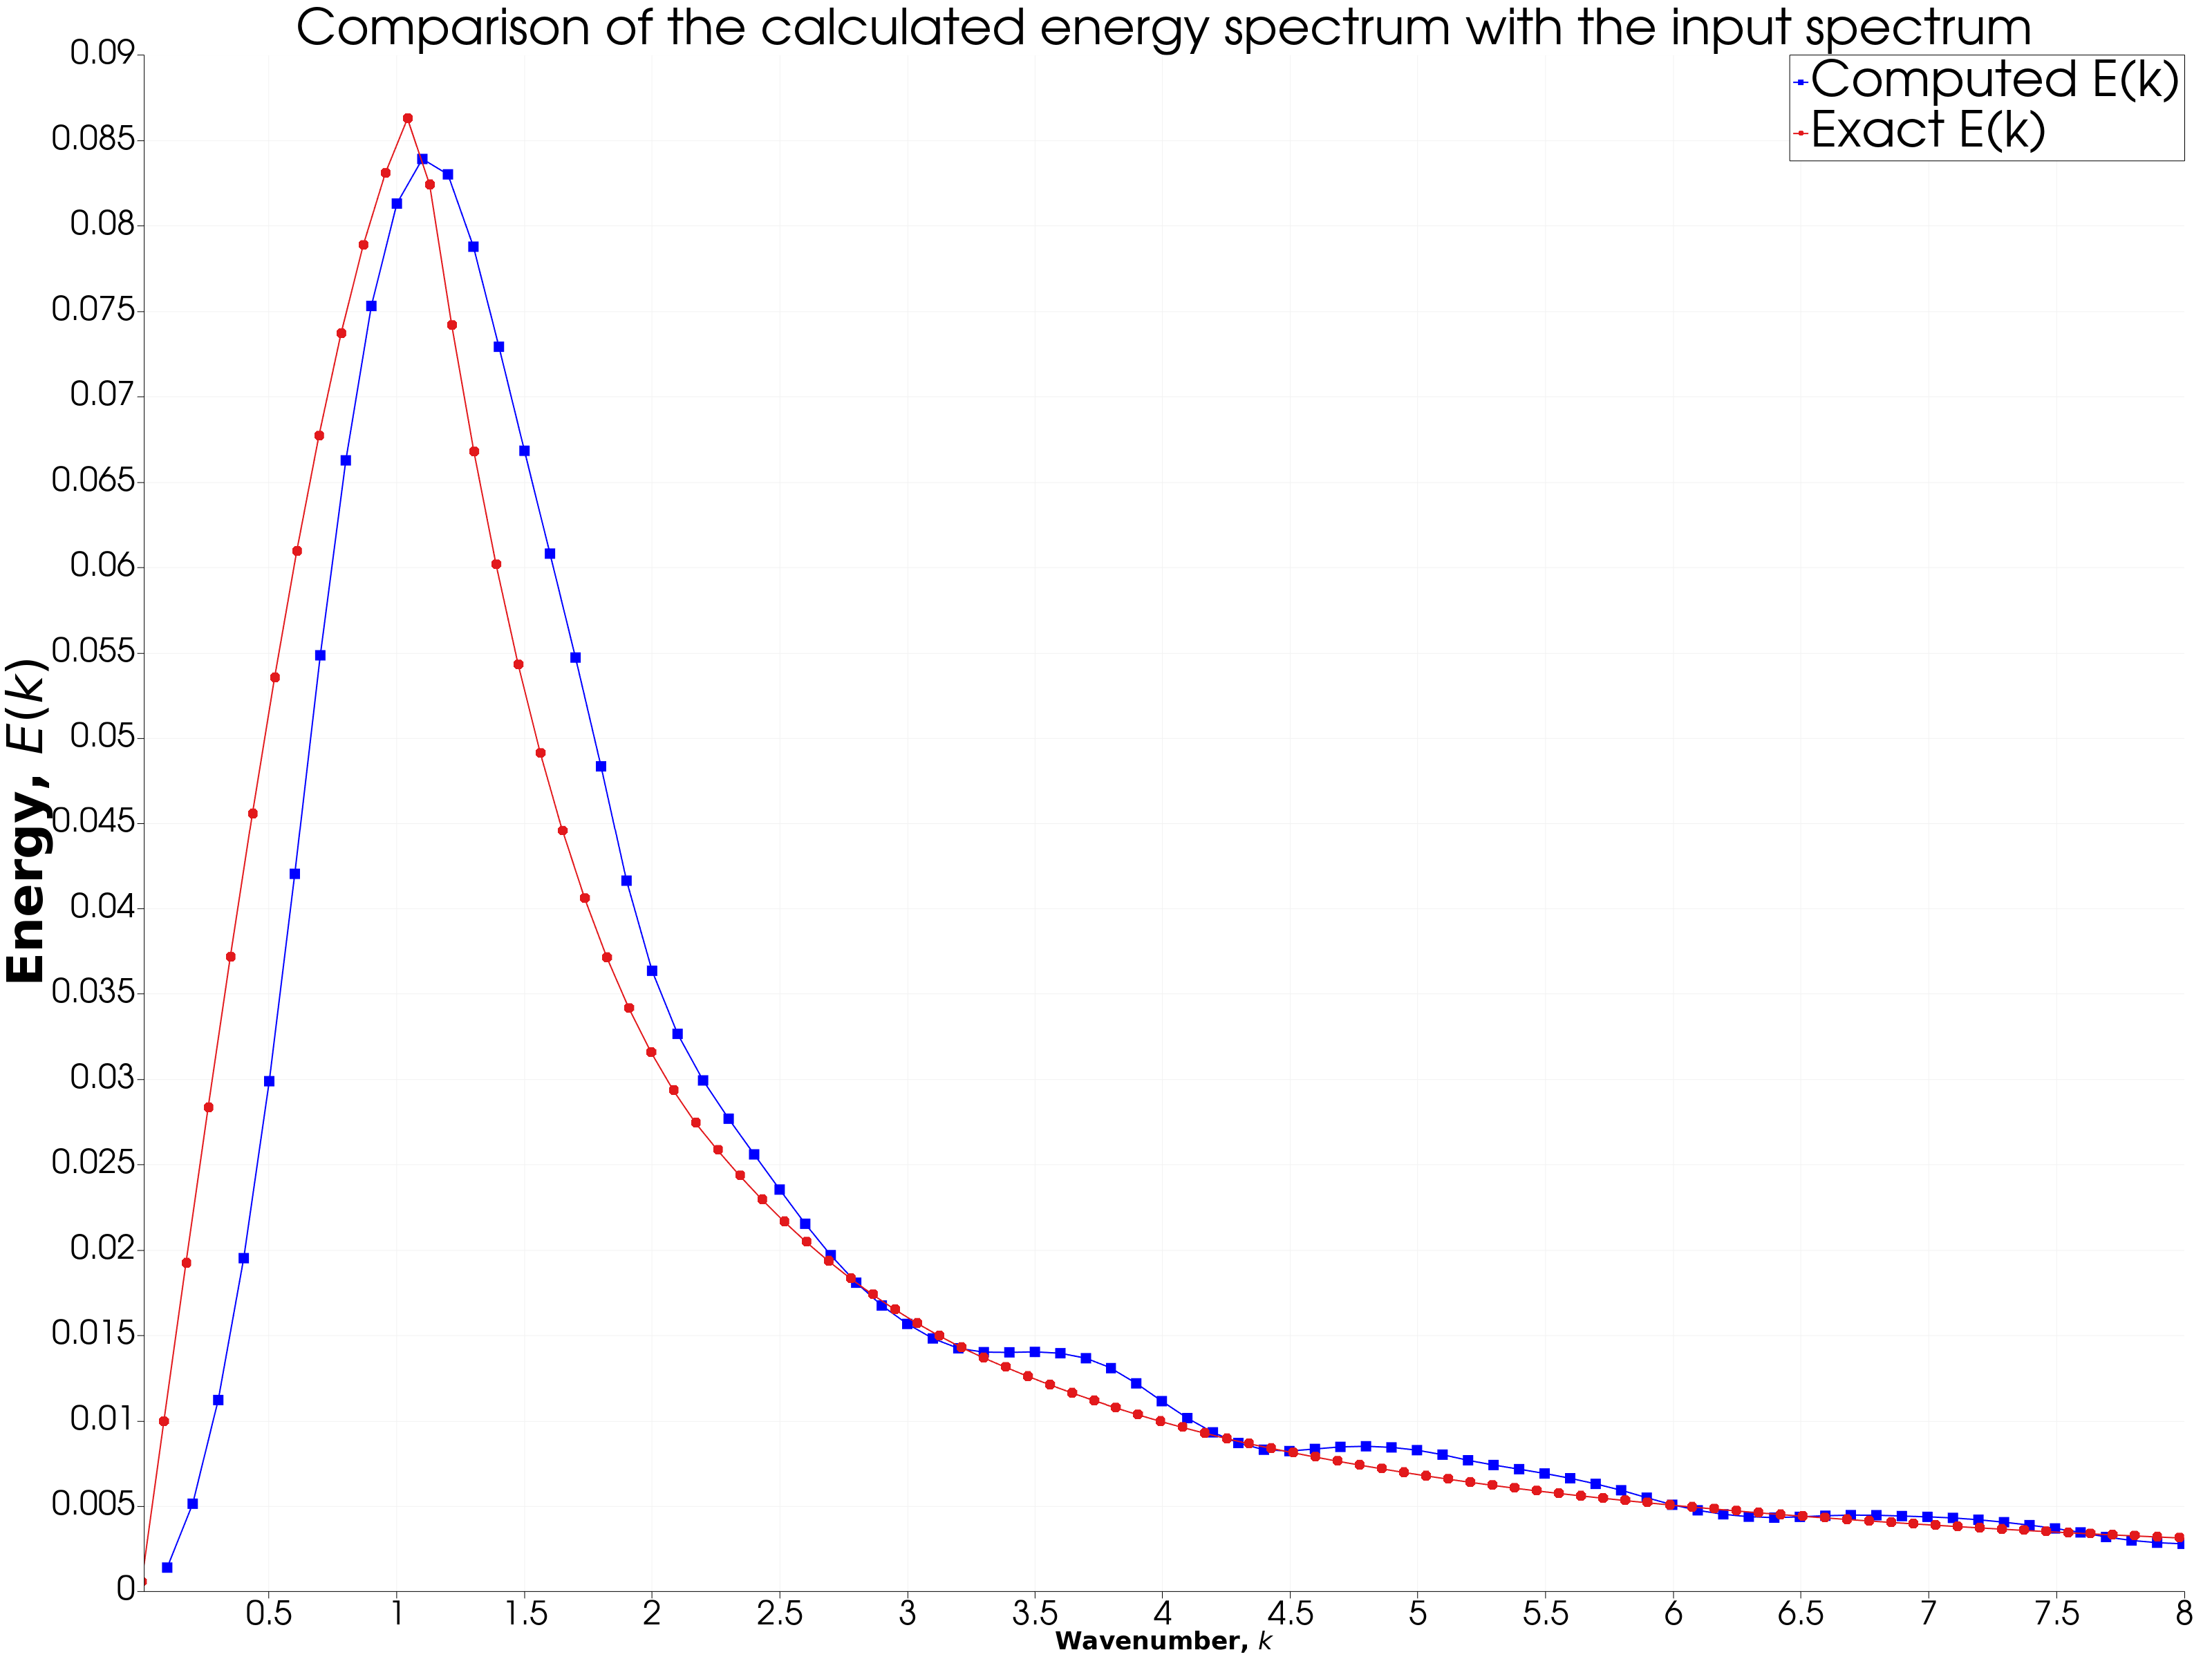
\includegraphics [width=0.8\linewidth] {images/spectral/spectra_l10_k10_f1000_n51.png}
    \caption{Сравнение энергетического спектра для предлагаемой модиификации спектрального метода с задаваемым.} 
    \label{img:spectral_desam_spectra_comarison}  
\end{figure}

\begin{figure}[ht] 
    \center
    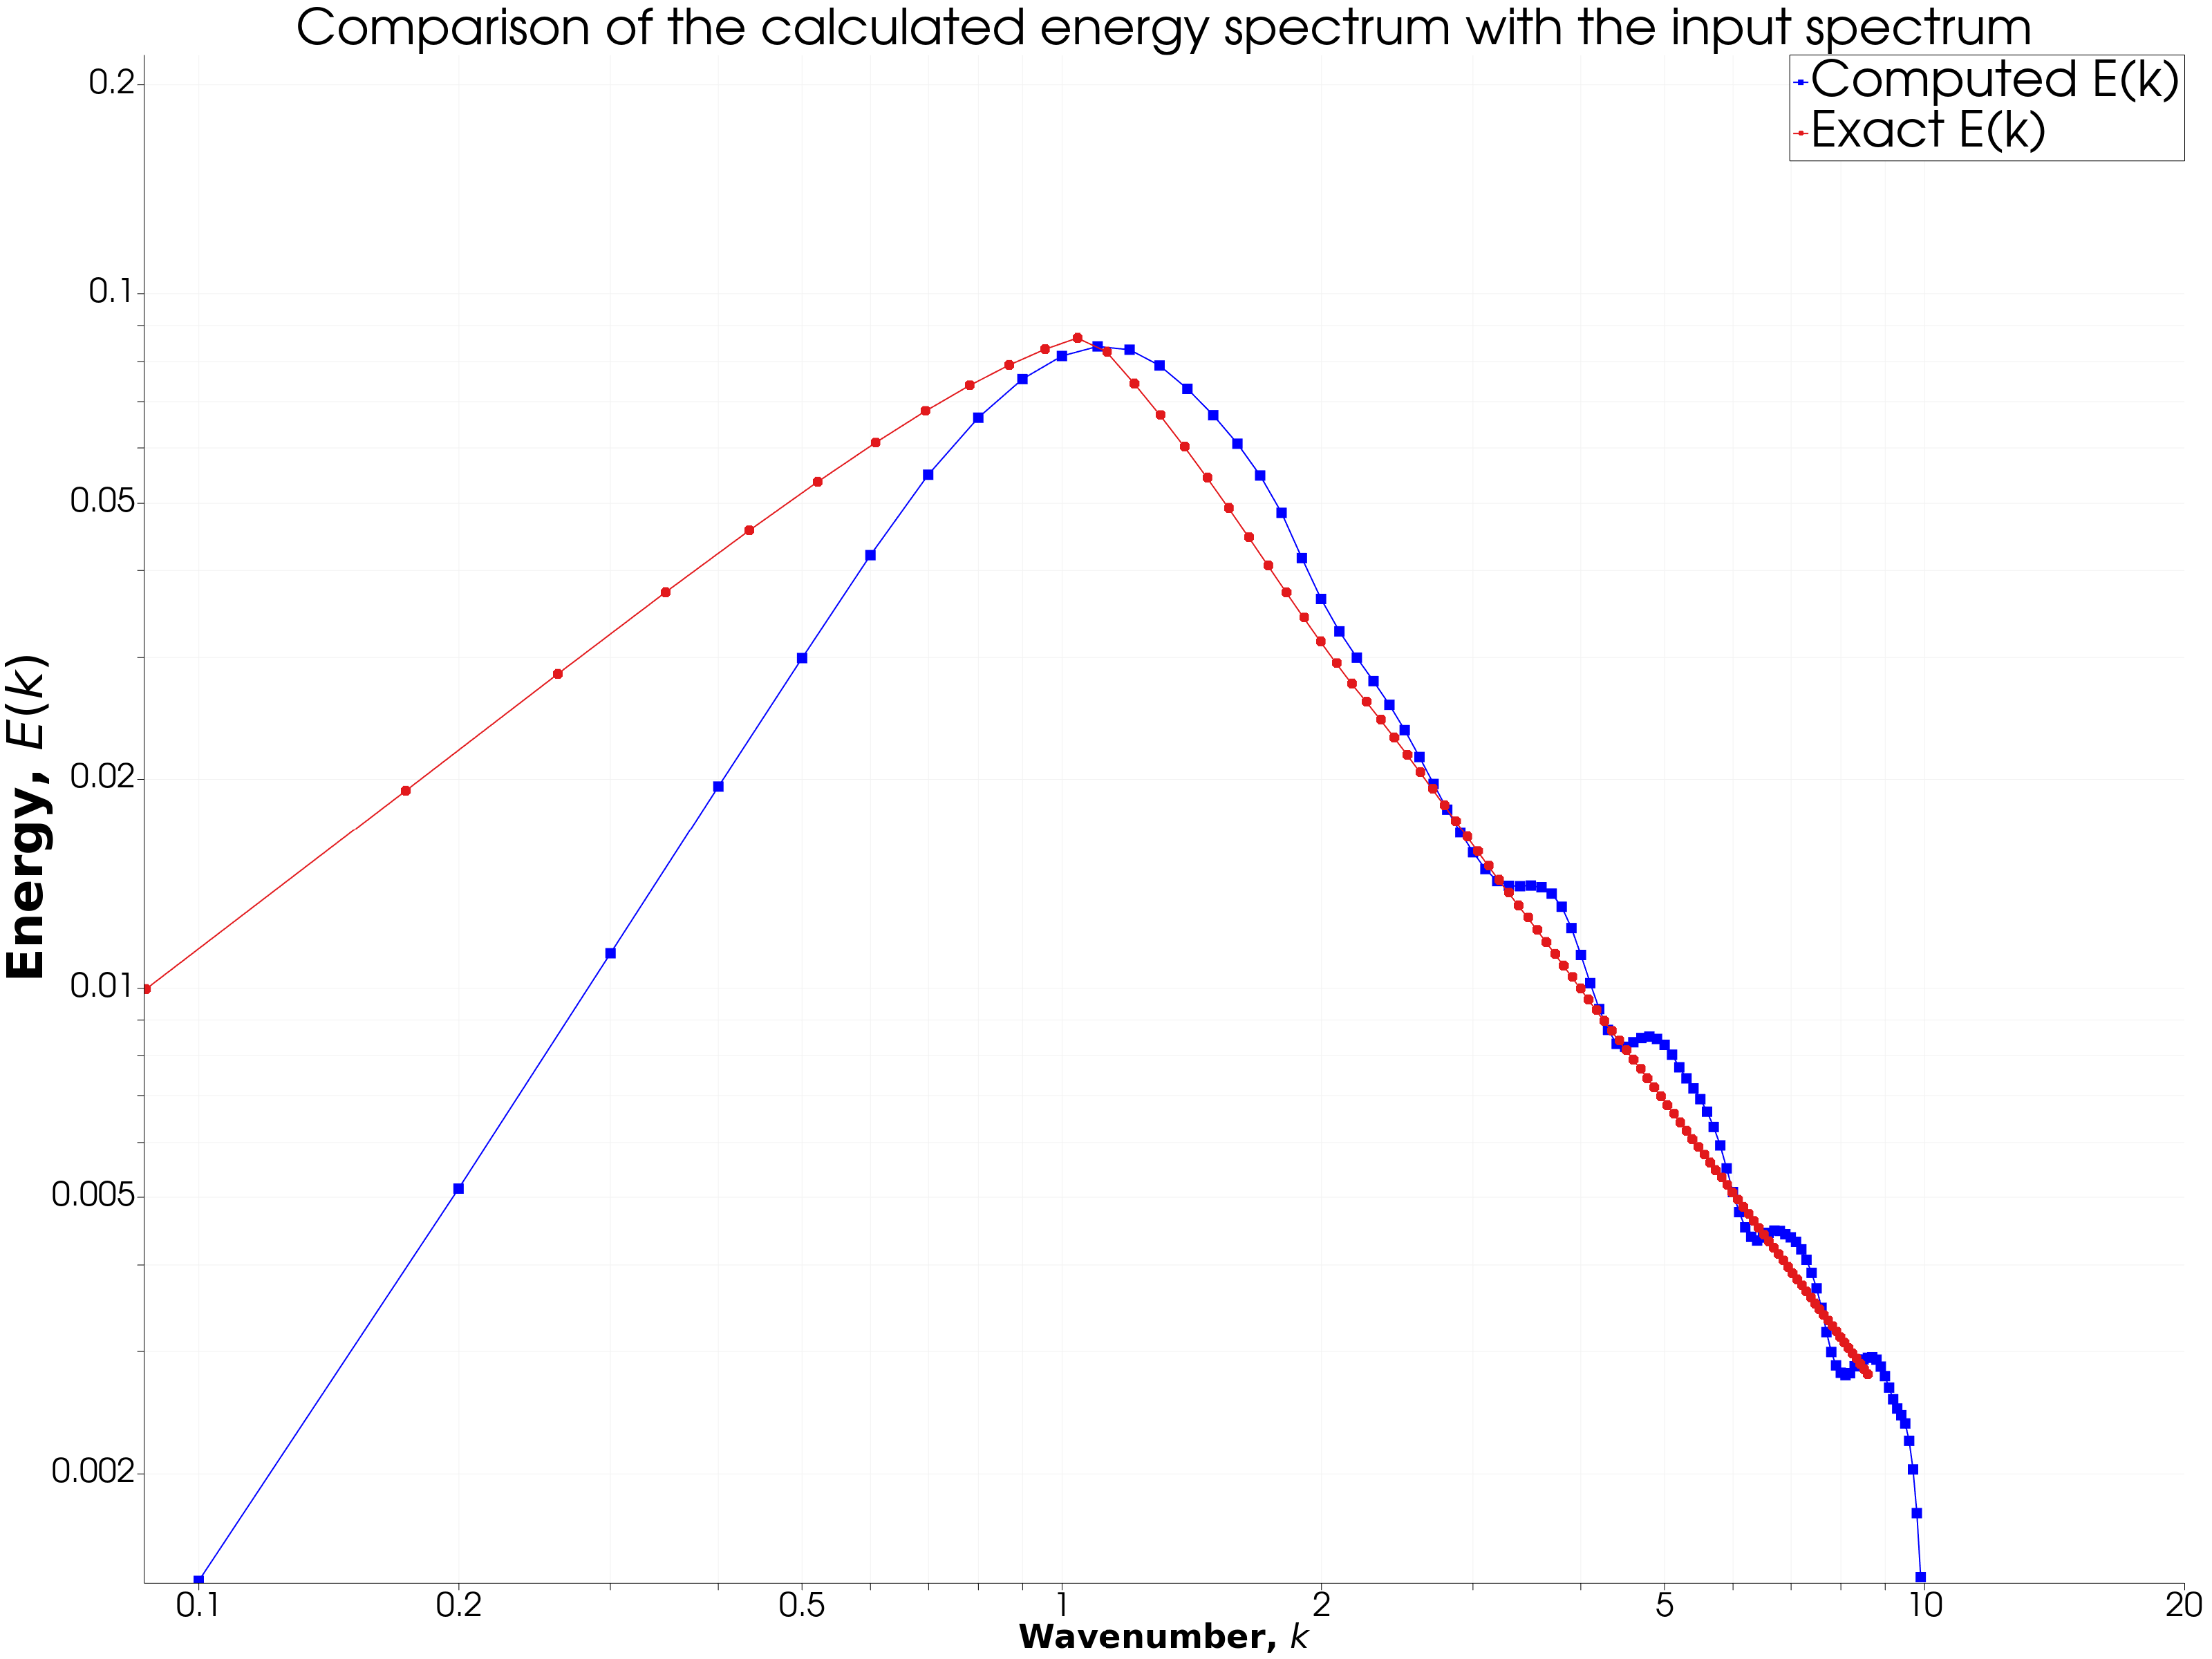
\includegraphics [width=0.8\linewidth] {images/spectral/spectra_l10_k10_f1000_n51_loglog.png}
    \caption{Сравнение энергетического спектра для предлагаемой модиификации спектрального метода с задаваемым в логарифмических координатах} 
    \label{img:spectral_desam_spectra_comarison}  
\end{figure}

Во первых заметим большую разницу для малых значений волнового числа, связанное с тем что минимальное волновое число меньше чем волновое число для рассматриваемой сетке, в своб очередь в диапазоне начиная с минимального для сетки волнового числа наблюдается хорошее совпадение с целевым спектром, особенно в инерционном интервале, с хорошо известным законом $-\dfrac{5}{3}$.
  
\begin{figure}[ht] 
    \center
    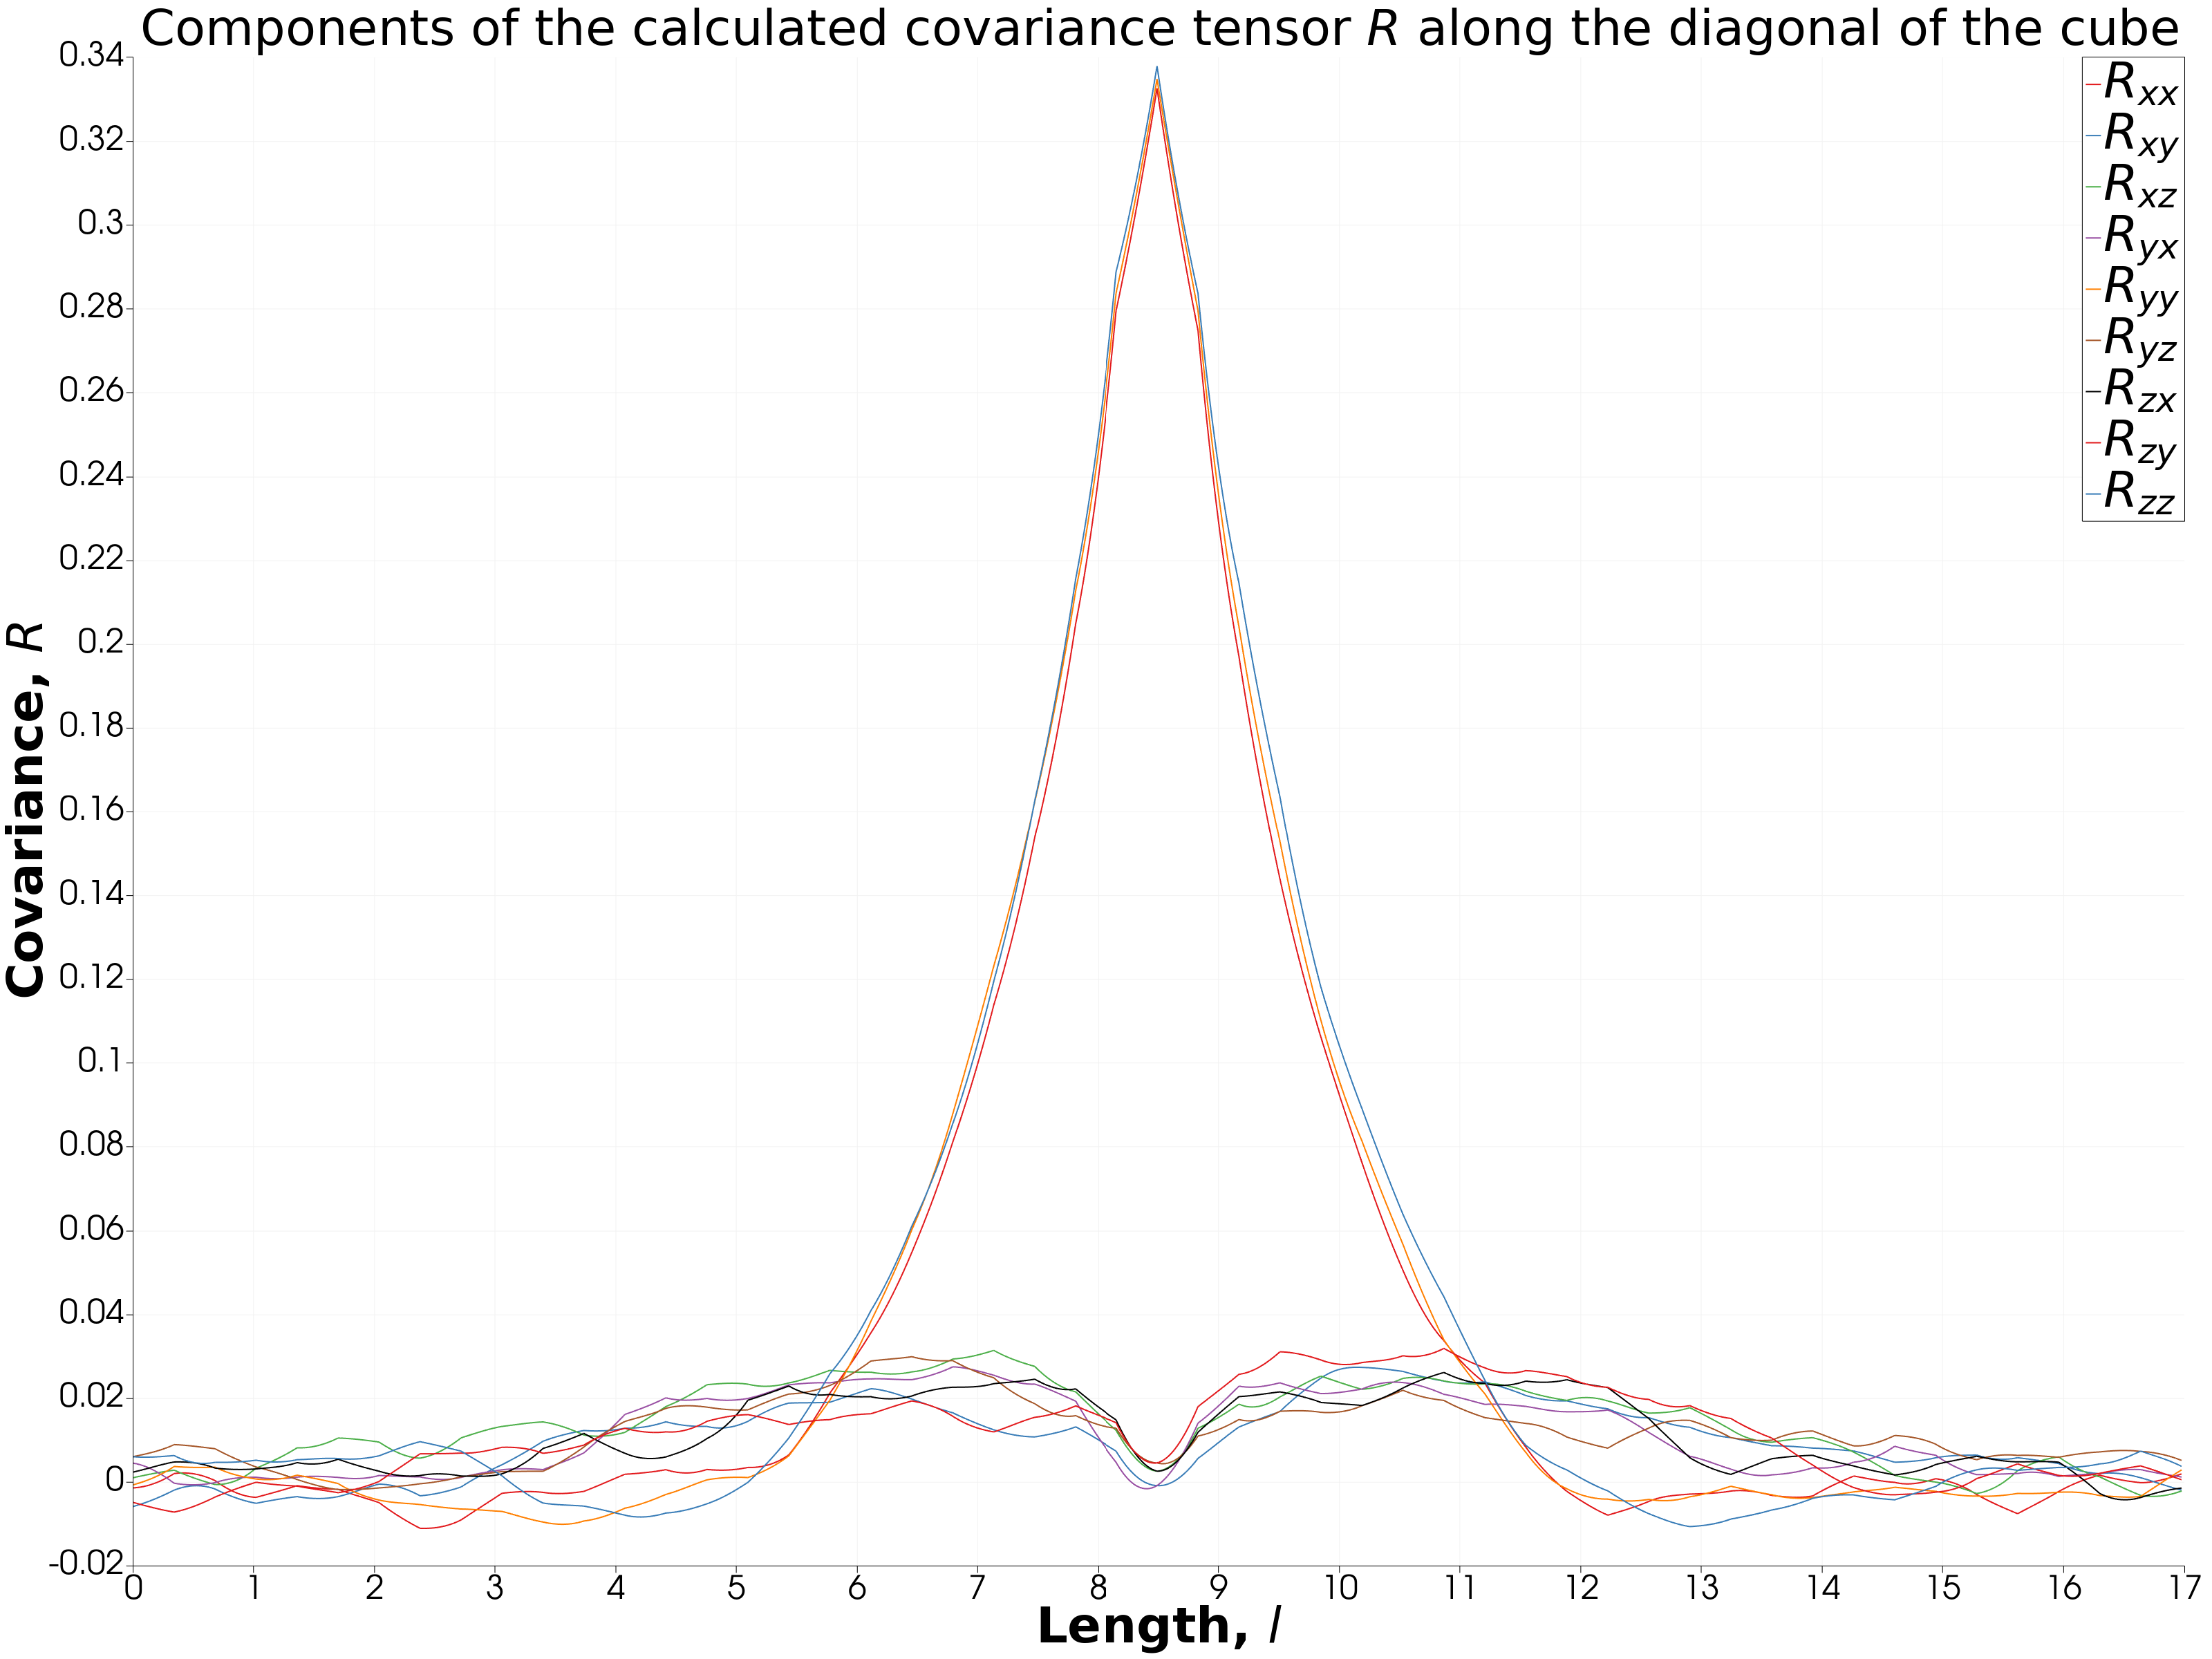
\includegraphics [width=0.8\linewidth] {images/spectral/covariance_function_tensor.png}
    \caption{Компоненты тензора ковариаций дволь диагонали вычислительной области} 
    \label{img:spectral_desam_covariance_comarison}  
\end{figure}

Сразу можно заметить, что по сравнению с генерацией на одной частоте, а именно методом Крайшнана, амплитуда ковариаций уменьшая бустрее с ростом расстояния от центра расчёта ковариации. Также уменьшилось расстояние на котором сохраняется пространственная ковариация двух величин, как было показано ранее, функция ковариации при генерации одной амплитуды сохраняет ковариацию на больших расстояниях, и имеет форму модулированной волны, в рассматриваемом сейчас случае, при достижении амплитуды ковариации при дальнейшем увеличении расстояния скоррелированость величин остаяется близи 0.

Приведём несколько сгенрированных полей флуктуаций с использованием предложенного метода. На рисунках ниже представлено по 3 плоскости с отображением направлений флуктуаций, для того чтобы показаться изменение векторов не только в плоскости $yz$ по нормали к оси $x$, центр поддомена совпадает с центром расчётной области.


\begin{figure}[ht] 
    \center
    \includegraphics [width=0.8\linewidth] {images/spectral/field_on_x_normal_yz_plane.png}
    \caption{Сгенерированное поле флуктуаций модифицированным методом, длины векторов пропорциональны длине векторов флуктуаций} 
    \label{img:spectral_result_field_no_angle}  
\end{figure}

\begin{figure}[ht] 
    \center
    \includegraphics [width=0.8\linewidth] {images/spectral/field_on_angle.png}
    \caption{Сгенерированное поле флуктуаций модифицированным методом, длины векторов пропорциональны длине векторов флуктуаций} 
    \label{img:spectral_result_field_on_angle}  
\end{figure}

На представленых рисунках хорошо видно вихревое движение во всех направлениях. За счёт пропорциональности длины векторов мы можем явно качественно разделить течение на зоны. 

Для сравнения методов по производительности использовалась сетка размерностью $n = 31$ и размером $l=10$. Для спектрального метода использовалось 1000 мод фурье с покрытием всего интервала волновых чисел, с такими параметрами достигается максимальная производительность не в угоду точности. Замер среднего времени генерации проводился на 1000 генераций. Полное время, потребовавшееся для генерации 1000 реализаций составило в среднем ~44 секунды, среднее время для генерации одной реализации поля скорости $\frac{44}{1000} \ approx 0.044$, принебрегая временем на операции записи результатов в файл.

